\chapter{FOSS projects as Cohesive Small Worlds}

As discussed in chapter \ref{collaborative_communities}, we named ``collaborative small world'' the network model that we propose in order to theoretically understand the structural dimension oc cooperation of FOSS projects. We argued that the family of networks that fit in the intersection of small world networks and structural cohesion networks exhibit consistent topological patterns. These patterns, we argue, provide the scaffolding for the emergence of collaborative communities. On the one hand, the generation of trust and congruent values among heterogeneous individuals are fostered by structurally cohesive groups in the network that play a key role in amplifying the effects of social interactions trough relatively long paths. On the other hand, the existence of highly connected local clusters linked together by relativelly small paths ---compared to suitable random networks--- allows successful collaboration among heterogeneous individuals with common interests even though they geographically dispersed and might never meet face to face.

This chapter focus on the empirical analysis of the network structure of two mature and well stablished FOSS projects: the CPython reference implementation of the Python programming language and the Debian Operating System. These two projects, as outlined in the previous chapter, are quite different despite being both successful FOSS projects. The Debian project has approximately ten times more participants than Python. Debian, being a complete Operating system, has many parts which are only lightly related between them becuse it contains programs that do very different tasks (eg the developers working on packaging software for music editing do not need to pay close attention to what devian developers focused on packaging word processors do). On the other hand, the Python programming language is a much more integrated software projects, and thus developers working on different parts of the language implementation have to play attention, and work very closely, with other developers.

This has a strong impact in the structure of the patterns of relations that emerge between developers in the two projects. The analysis presented here has two parts: first we will compute the small world metrics for the two projects, as described in chapter \ref{collaborative_communities}, and then we will compute the structural cohesion metrics as described in the chapter \ref{structural_cohesion}. However first we have to define how we build the networks for this two projects as a formalizations of the patterns of cooperation between the individuals in these projects.

\section{Modeling patterns of cooperation as networks}

Our modeling strategy to capture the patterns of relations among developers in these two projects is to focus on the actual contributions of each developer to the project. We model the cooperation patterns between individuals as affiliation networks \citep[chapter 8]{wasserman:1994}. This kind of networks contain two types of nodes: $N$ actors each of which belongs to one or more groups $M$. Such networks are bipartite or 2-mode because they contain two types of nodes and there are no edges between nodes of same type.

The two sets of nodes in the networks analyzed here are, on the one hand, human developers and, on the other hand, entities that conform the product that is released by the FOSS project. In the case of Debian, these entities are software packages, and in the case of Python, they are source code files. Note that the collaboration network is based on individual contribution but it not only captures the total amount of contribution that a given individual does, but also to which part of the project the contributions are focused, and who else in the project is also working on the same entities. This is why we name these bipartite graphs collaboration or cooperation networks.

One feature of most large software projects is modularity, that could be defined as the division of a software project into semi-independent parts, designed to work together but that can be developed relatively independently. In the case of an operating system, such as the Debian project, modularity is more important than in other software projects, such as Python. An operating system comprises a comprehensive set of software packages with varying importance, from those responsible for interacting with the hardware to others that provide certain features that are only useful in very specific and specialized configurations. On the other hand, an implementation of a programming language, such as Python, is also modular but their parts are much more closely related and have to be tightly integrated in order to function as a coherent whole.

This modeling approach captures mostly the informal patterns of relations that individuals establish when contributing to the project. FOSS projects have a wide range of formal organizational forms, and in this respect, they can be quite different. The definition of the leadership position in the two projects in which we focus this thesis nicely capture these differences in formal organization: Debian has a very developed formal bureaucracy, the project elects its leader each year through a secret vote of all its members after a electoral campaign where the candidates discuss among them and try to gain supports; Python instead has its original author ---Guido van Rossum--- in a permanent position of leadership, the people in the project refer to him, and his position of leadership, as ``Benevolent Dictator For Life'' (BDFL).

Despite these differences in the formal organization, if we focus on the patterns of relations among developers in the productive process, what we call the cooperation network, we can analyze the contribution dynamics, analyze hierarchical positions defined by these patterns, assess the pace of renewal in these positions, and determine the impact in the median active life on a developer in a project of being in a concrete hierarchical position.

For the case of the Debian project, we define that each package of source code is a module of the system or, in terms of network affiliation, a group or team. The main data source is the Ultimate Debian Database (UDD)\footnote{\href{http://udd.debian.org/}{http://udd.debian.org/} [accessed November 2016]} \citep{udd:2010}. The UDD contains information related to the work of each individual in the project which allow us to build the developers-packages affiliation network. One developer is linked to every package she has uploaded in the archive in a period of one year. Therefore, the result is a 2-mode network with developers ---the actors--- and packages ---the groups--- as the two types of nodes.

For the case of the Python project, we define that each source code file that forms the reference implementation of the programming language is a module of the system or, in terms of network affiliation, a group or team. Thus, contributions are lines of source code added or deleted from one of the source code files of Python's code base. The main data source is the Python source code repository \footnote{\href{https://hg.python.org/}{https://hg.python.org/} [accessed November 2016]}, which is under version control. That means that each change to any source code file is recorded and attributed to a person.

These collaboration relations are only part of the whole patterns of cooperative relations established among developers in both projects. We cannot obtain more accurate data of the frequent interactions between developers related to the production process that take place in a large variety of on-line or face-to-face settings. However, the subset of collaboration relations captured by our approach are significative and serve our purpose to analyze the global patterns of relations among direct producers because the result of the productive process is, in fact, the archive of packages that form the Debian operating system or the set of source code files taht form the implementation of the Python programming language. Therefore, we base our analysis of cooperation on the registered contribution of each developer to the final product of the productive process delivered to end users.

Moreover, two important advantages of this approach are, on the one hand, that we have data on all uploads ---in the case of Debian--- or all the modifications of source code files ---for the Python project---, thus we do not need to worry about sample bias because we have accurate data of all the work performed in the period under analysis. On the other hand, we have a strict definition of what cooperation means, which allow us analyze the evolution of collaboration patterns throughout the history of the two projects. Therefore, we can make meaningful comparisons between years in the same project, and between projects.

\subsection{Null models}

Both kinds of analysis presented in this chapter have in common the use of null models. In empirical analysis of networks we need to be able to compare the statistical measures obtained of our actual networks with a null model in order to assert that what we observe is not the result of pure chance. That is, we have to make sure that the metrics observed in the actual networks are significantly different to the patterns of relations that we might expect if the relation between developers and packages, or developers and files in the case of Python, were produced uniformly at random.

To this end, the canonical approach is to compare the measures of actual networks with measures taken from random networks that maintain some constraints of the original network, such as the degree distribution. \citet*{newman:2003,nsw:2001} provided a configuration model in order to generate random graphs with arbitrary degree distributions. In the analysis presented here we have used the configuration model for 2-mode networks to generate 100 random null models for each year. The configuration model assigns at random developers to packages, or developers to source code files, maintaining the concrete skewed distribution of packages by developer and files by developer observed in the actual networks.

\section{Small World Metrics}

As we discussed in chapter \ref{collaborative_communities}, a network fits the small world model if it is more clustered ($CC$) than its random network counterpart but has approximately the same average distance ($L$) between nodes. In unipartite or 1-mode networks, $CC$ is the mean probability that two nodes that are neighbors of the same other node will themselves be neighbors. Thus, this measure is computed as the ratio of triangles ---a fully connected graph of 3 nodes--- over two-stars ---three nodes connected by two edges---. But, in bipartite or 2-mode networks there can be no triangles because, by definition, edges can only link nodes of different type. Following \citet{robins:2004}, \citet{lind:2005} and \citet{latapy:2008}, local cohesion in 2-mode networks can be measured with the notion of cluster coefficient based on squares ($CC_4$). $CC_4$ is the ratio between the number of squares ($C_4$) ---composed by two nodes of each type linked by four edges--- over the number of three-paths ($L_3$) ---composed by two nodes of each type linked by three edges--- (See appendix \ref{sw-affnets} for a formal definition of $CC_4$). Like $CC$, $CC_4$ applied to bipartite networks is a measurement of local cohesion.

The Small World Index ($Q$) is a summary indicator of the smallworldiness of a network and accounts for both the relation of the clustering coefficients of actual networks compared to their random counterparts, and the relation of average path length (a global measure of the average distance between nodes in a network) of actual networks compared to their random counterparts. Networks with the Small World Index ($Q$) bigger than 1 are considered small world networks (see appendix \ref{sw-affnets} for details). We compute the Small World Index using the following formulas:

\begin{equation}
% \begin{split}
Q = \frac{CC_{ratio}}{L_{ratio}}
% \end{split}
\end{equation}

Where:

\begin{align}
CC_{ratio}& = \frac{CC_{actual}}{CC_{random}} &
L_{ratio}& = \frac{L_{actual}}{L_{random}} \nonumber \\
\end{align}


In the first place we compute small world metrics for Debian networks. The results are shown in table \ref{swi_debian}.

\begin{table}
\begin{center}
\begin{tabular}{|c|c|c|c|c|c|c|c|c|c|}
\hline
Years&Nodes&Developers&Packages&Edges&CC&random CC&APL&random APL&SWI ($Q$)\\
\hline
1999&3258&391&2867&3250&0.127&0.002&9.4&8.8&54.4\\
2000&3590&521&3069&3493&0.136&0.002&9.5&8.9&80.4\\
2001&5921&755&5166&6158&0.050&0.001&8.4&7.9&31.9\\
2002&6839&840&5999&7109&0.079&0.001&9.2&8.0&48.3\\
2003&7244&882&6362&7764&0.102&0.002&9.0&7.7&56.9\\
2004&7971&982&6989&9390&0.155&0.002&8.0&6.6&52.3\\
2005&8317&1037&7280&10242&0.169&0.003&7.5&6.2&44.1\\
2006&9564&1127&8437&12863&0.173&0.005&6.7&5.6&31.7\\
2007&9434&1145&8289&12736&0.144&0.004&6.8&5.6&26.7\\
2008&10605&1212&9393&14226&0.188&0.004&7.1&5.6&33.1\\
2009&11284&1293&9991&15538&0.229&0.006&7.0&5.4&30.8\\
2010&10447&1319&9128&13702&0.282&0.005&7.7&5.6&40.2\\
2011&12265&1333&10932&15862&0.141&0.005&7.5&5.5&21.3\\
2012&8408&1055&7353&9528&0.162&0.003&9.5&6.2&32.9\\
\hline
\end{tabular}
\caption{Small world metrics for debian networks.}
\label{swi_debian}
\end{center}
\end{table}



As we can see, the Debian project cooperation networks for all years analyzed are indeed small world networks. Their Small World Index ($Q$) is way bigger than 1, ranging from 21 in 2011 to 80 in year 2000. This large value of $Q$ is driven by the fact that the clustering coefficient ---the measure of local cohesion--- of the observed networks is approximately a hundred times higher than in their random counterparts. However the average distance between nodes in the actual networks is slightly higher than the distance in their random counterparts, which reduces the value of the small world index. Therefore we can conclude that Debian cooperation networks fit nicely the small world model. 

For the Python project, the results for the small world metrics are presented in table \ref{swi_python}.

\begin{table}[H]
\begin{center}
\begin{small}
\begin{tabular}{|c|c|c|c|c|c|c|c|c|c|}
\hline
Years&Nodes&Developers&Files&Edges&CC&random CC&APL&random APL&SWI ($Q$)\\
\hline
1999&1,146&9&1,137&1,236&0.102&0.039&3.1&3.5&3.0\\
2000&2,172&31&2,141&3,720&0.214&0.135&3.3&3.5&1.7\\
2001&2,511&33&2,478&4,507&0.205&0.129&3.4&3.6&1.7\\
2002&2,317&38&2,279&4,502&0.204&0.129&3.6&3.6&1.6\\
2003&1,805&42&1,763&3,192&0.153&0.112&3.5&3.6&1.4\\
2004&1,850&49&1,801&3,163&0.113&0.093&3.4&3.6&1.3\\
2005&1,007&44&963&1,759&0.129&0.079&3.7&3.7&1.7\\
2006&2,632&52&2,580&6,794&0.235&0.156&2.8&3.2&1.7\\
2007&3,359&51&3,308&7,790&0.223&0.177&2.9&3.3&1.4\\
2008&2,951&59&2,892&7,833&0.231&0.175&3.0&3.3&1.5\\
2009&2,219&58&2,161&4,708&0.228&0.142&3.1&3.4&1.7\\
2010&2,930&63&2,867&6,504&0.175&0.128&3.4&3.5&1.4\\
2011&2,174&63&2,111&4,459&0.145&0.114&3.5&3.6&1.3\\
2012&2,444&65&2,379&4,843&0.124&0.087&3.7&3.8&1.4\\
2013&2,285&63&2,222&4,743&0.147&0.099&3.6&3.7&1.5\\
2014&2,134&62&2,072&4,149&0.138&0.095&3.6&3.7&1.5\\
\hline
\end{tabular}
\caption{Small world metrics for python networks.}
\label{swi_python}
\end{small}
\end{center}
\end{table}





\section{Structural Cohesion Metrics}

\begin{table}[H]
\begin{center}
\begin{tabular}{|c|c|c|c|c|c|c|c|}
\hline
Years&Nodes&GC&Random GC&GBC&Random GBC&maximum $k$&Random max $k$\\
\hline
1999&1146&66.0\%&100.0\%&6.7\%&6.5\%&3 (1.0\%)&2 (6.5\%)\\
2000&2172&96.5\%&100.0\%&33.4\%&31.4\%&8 (1.2\%)&5 (3.1\%)\\
2001&2511&97.3\%&99.8\%&34.1\%&33.0\%&9 (1.2\%)&6 (2.4\%)\\
2002&2317&100.0\%&99.8\%&38.1\%&36.9\%&9 (2.6\%)&7 (1.9\%)\\
2003&1805&100.0\%&99.2\%&34.8\%&33.1\%&7 (3.3\%)&6 (2.4\%)\\
2004&1850&99.8\%&100.0\%&39.7\%&37.1\%&7 (1.8\%)&5 (2.5\%)\\
2005&1007&99.8\%&100.0\%&45.7\%&44.2\%&5 (5.8\%)&4 (7.6\%)\\
2006&2632&100.0\%&100.0\%&74.2\%&69.8\%&9 (1.5\%)&6 (3.9\%)\\
2007&3359&100.0\%&100.0\%&58.6\%&55.2\%&9 (2.0\%)&6 (2.2\%)\\
2008&2951&100.0\%&99.9\%&64.5\%&61.7\%&10 (2.2\%)&7 (2.5\%)\\
2009&2219&100.0\%&99.9\%&51.0\%&48.5\%&7 (2.8\%)&5 (5.6\%)\\
2010&2930&100.0\%&99.9\%&48.7\%&47.0\%&9 (2.7\%)&7 (2.4\%)\\
2011&2174&100.0\%&99.8\%&47.7\%&45.9\%&8 (2.9\%)&7 (1.7\%)\\
2012&2444&99.8\%&99.8\%&41.1\%&40.3\%&8 (3.4\%)&7 (3.4\%)\\
2013&2285&99.9\%&99.9\%&51.6\%&49.8\%&7 (4.2\%)&6 (4.0\%)\\
2014&2134&100.0\%&99.8\%&44.6\%&43.4\%&7 (2.6\%)&6 (3.1\%)\\
\hline
\end{tabular}
\caption{Structural Cohesion metrics for python networks.}
\label{str_cohesion_python}
\end{center}
\end{table}



\begin{figure}[p]
%\centering
\subfloat[Actual Python network 2000]{
\label{fig:s3d_actual_python_2000}
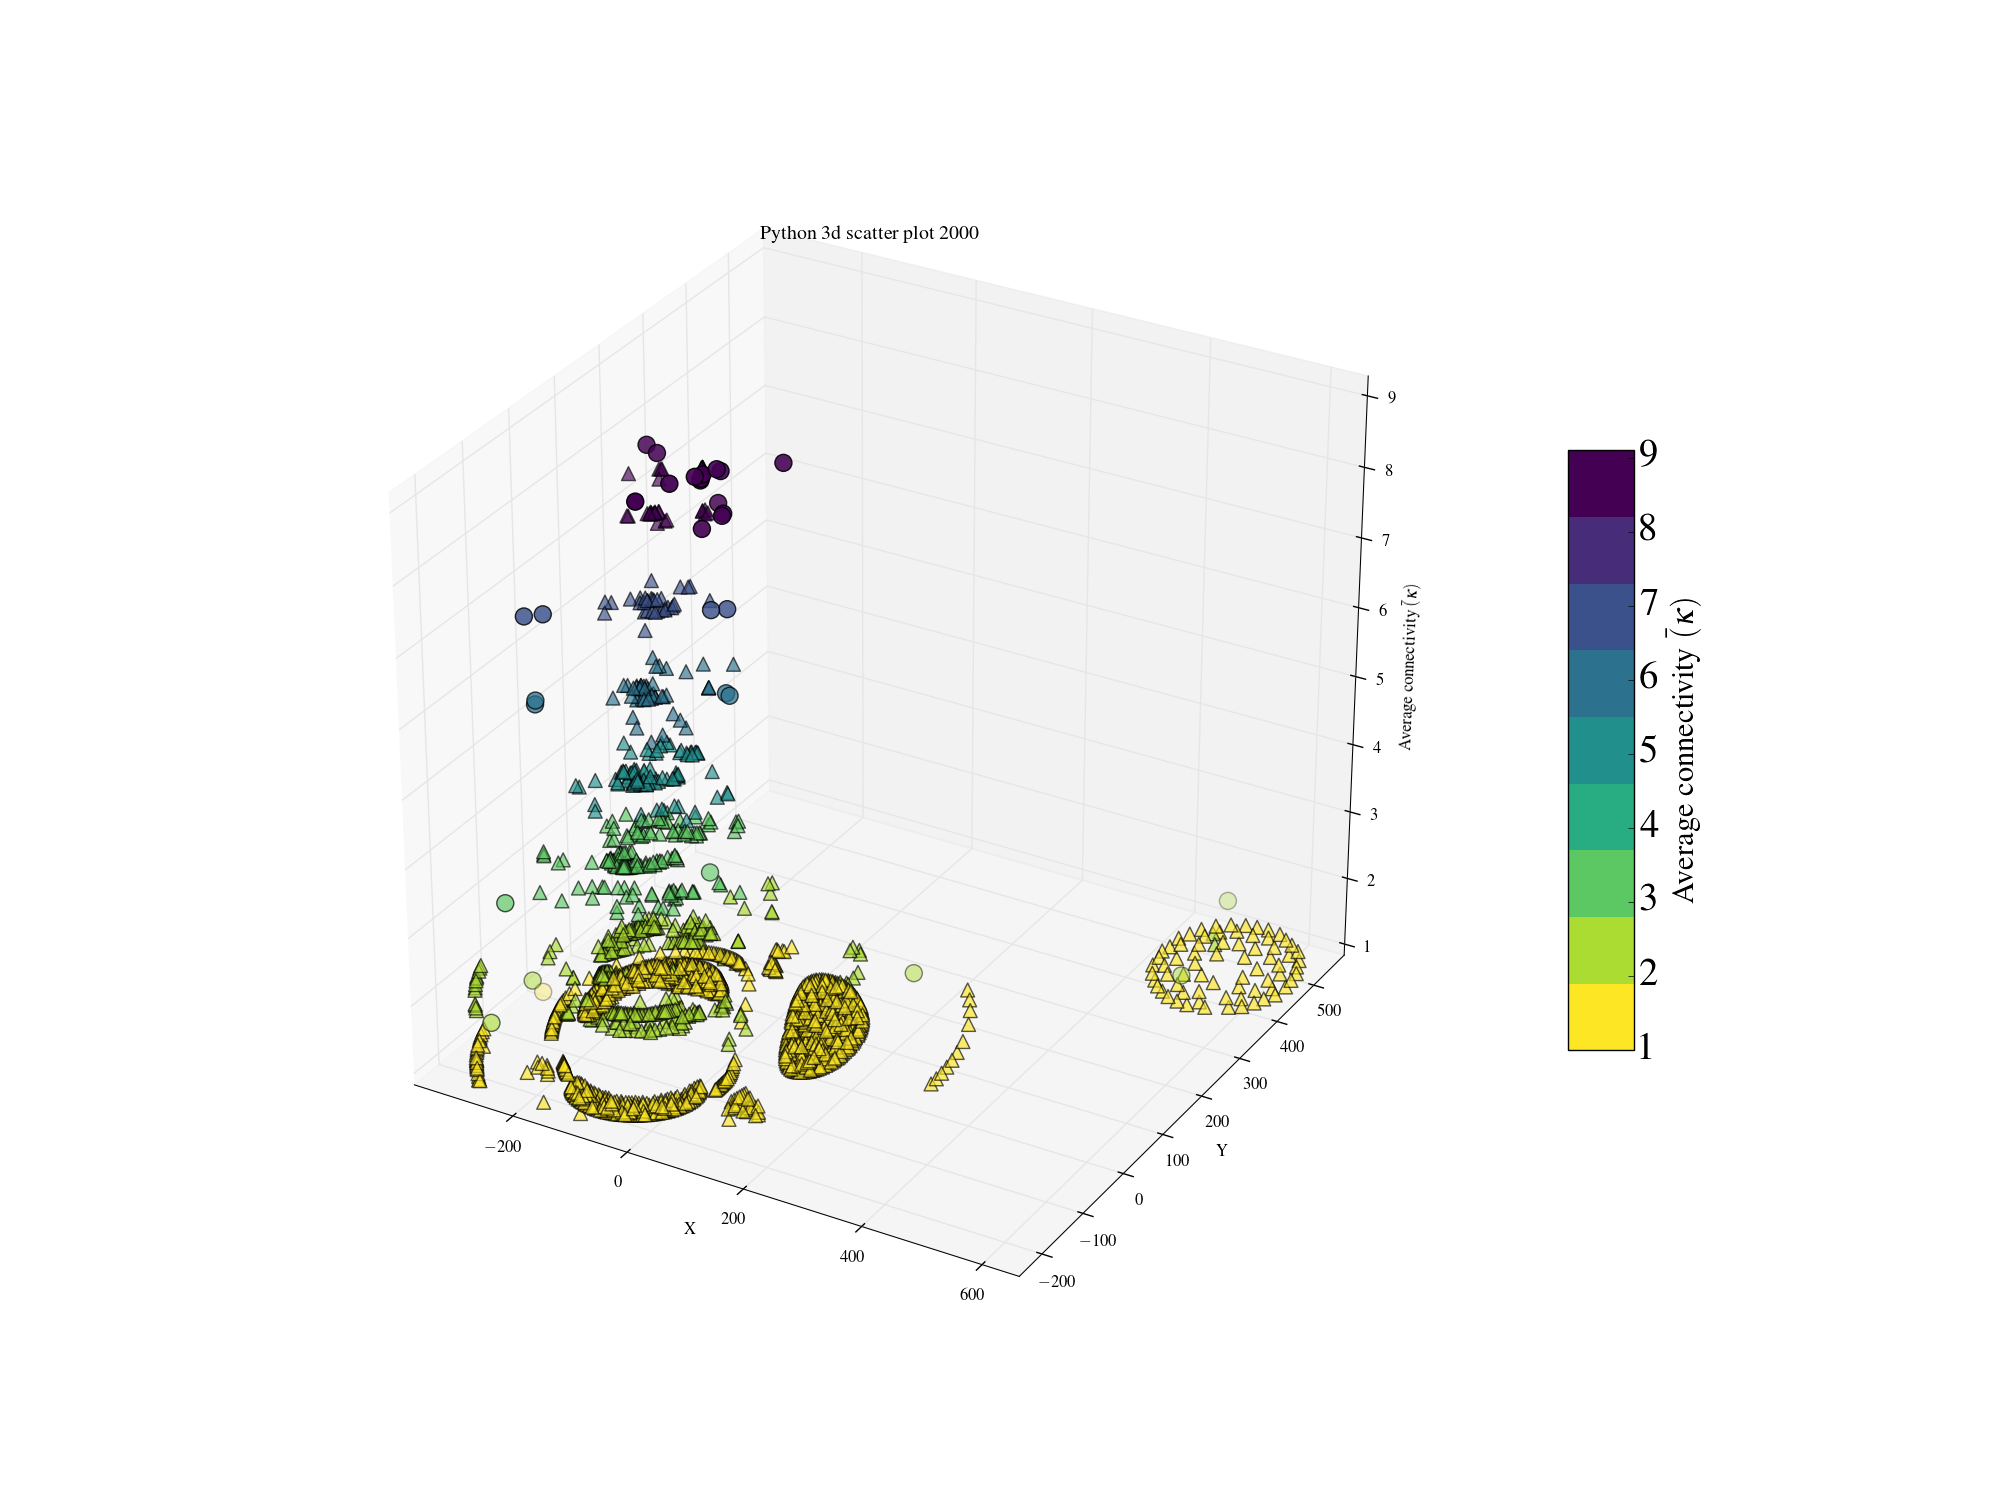
\includegraphics[scale=0.23]{figures/3d_scatter_python_2000}
}
\hspace{.01in}
\subfloat[Null model Python network 2000]{
\label{fig:s3d_null_python_2000}
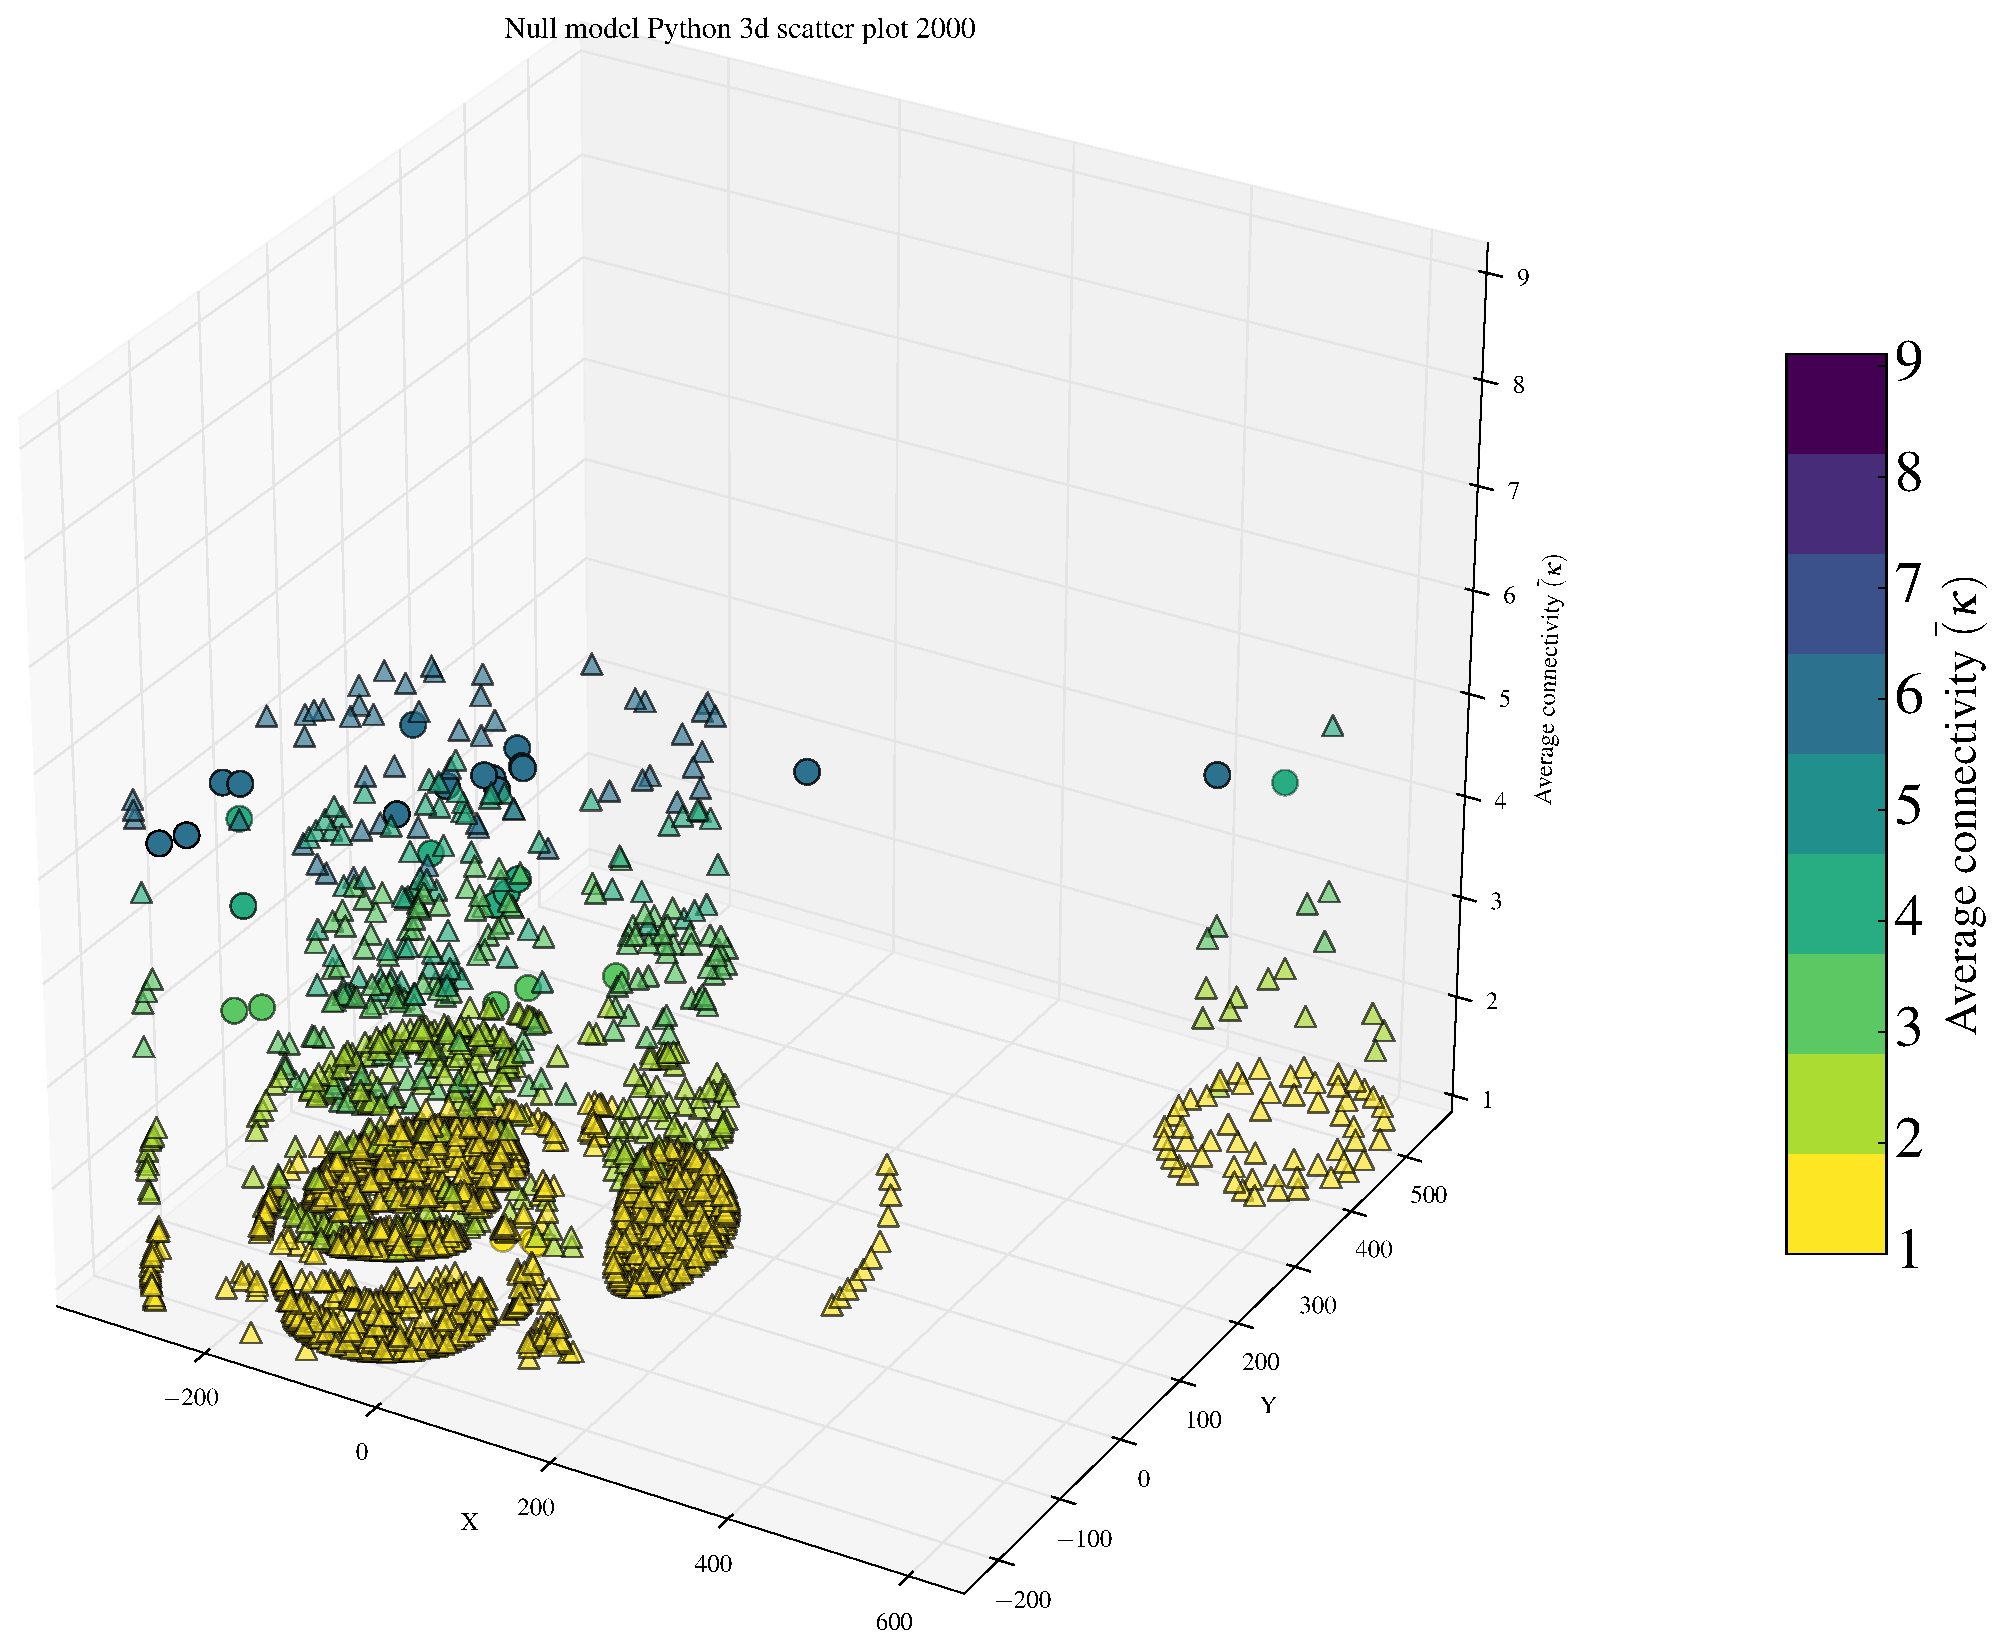
\includegraphics[scale=0.23]{figures/3d_scatter_python_2000_null}
}

\subfloat[Actual Python network 2004]{
\label{fig:s3d_actual_python_2004}
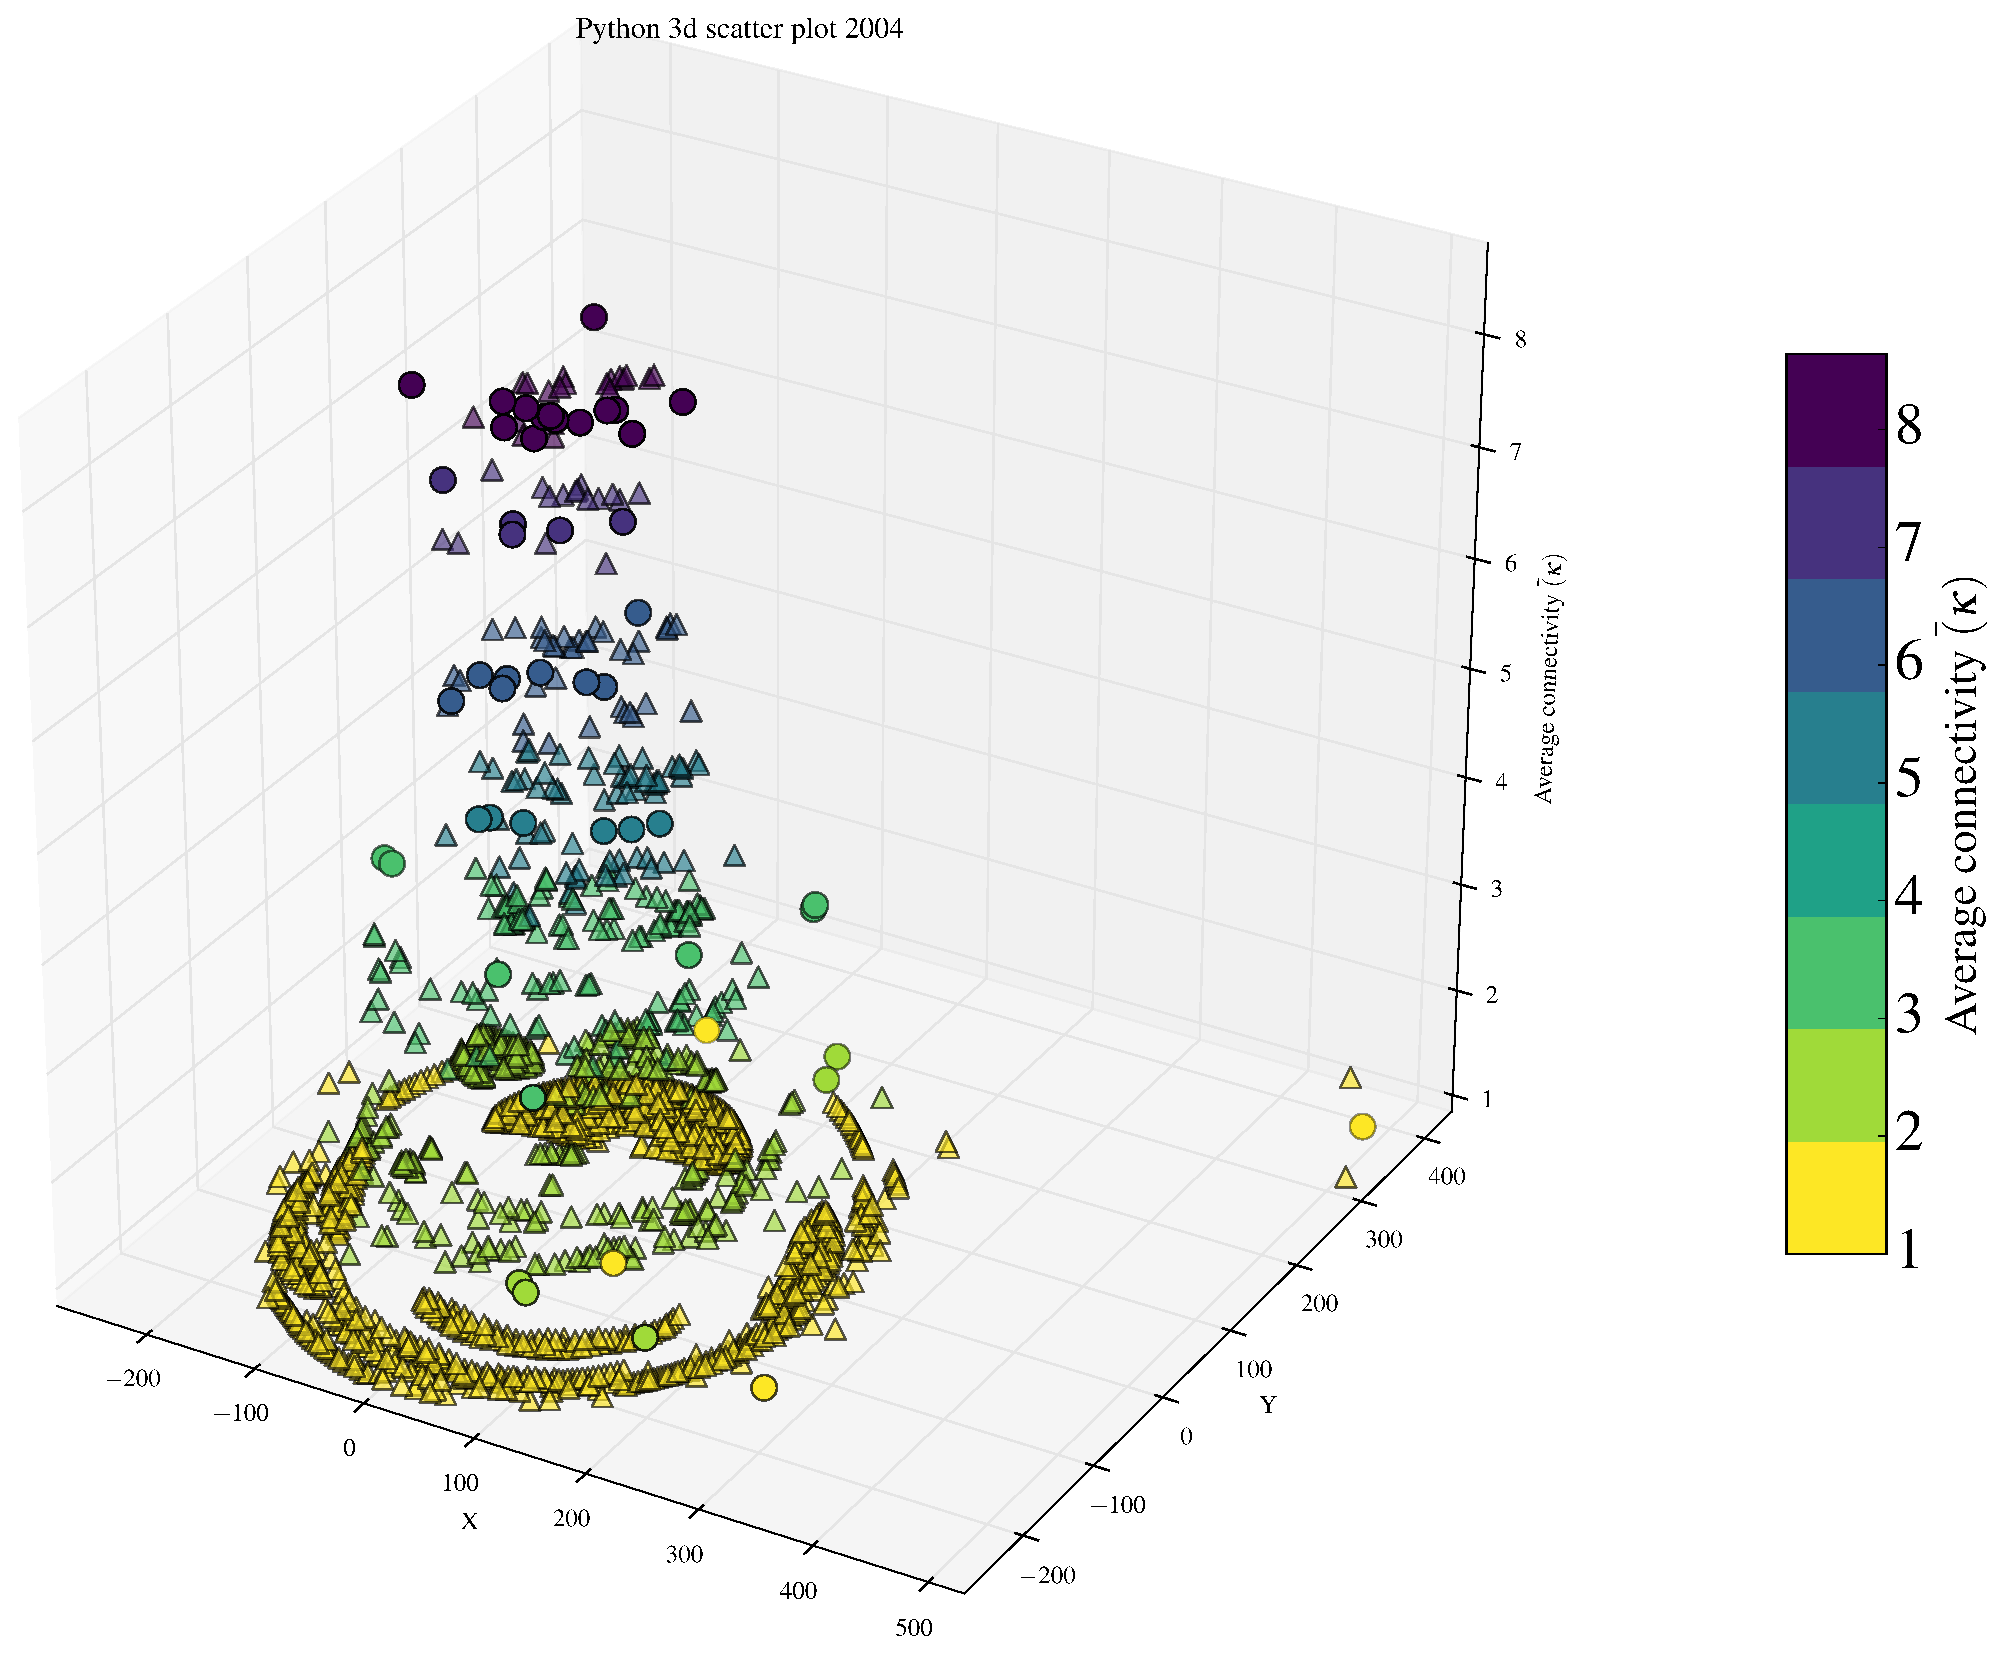
\includegraphics[scale=0.23]{figures/3d_scatter_python_2004}
}
\hspace{.01in}
\subfloat[Null model Python network 2004]{
\label{fig:s3d_null_python_2004}
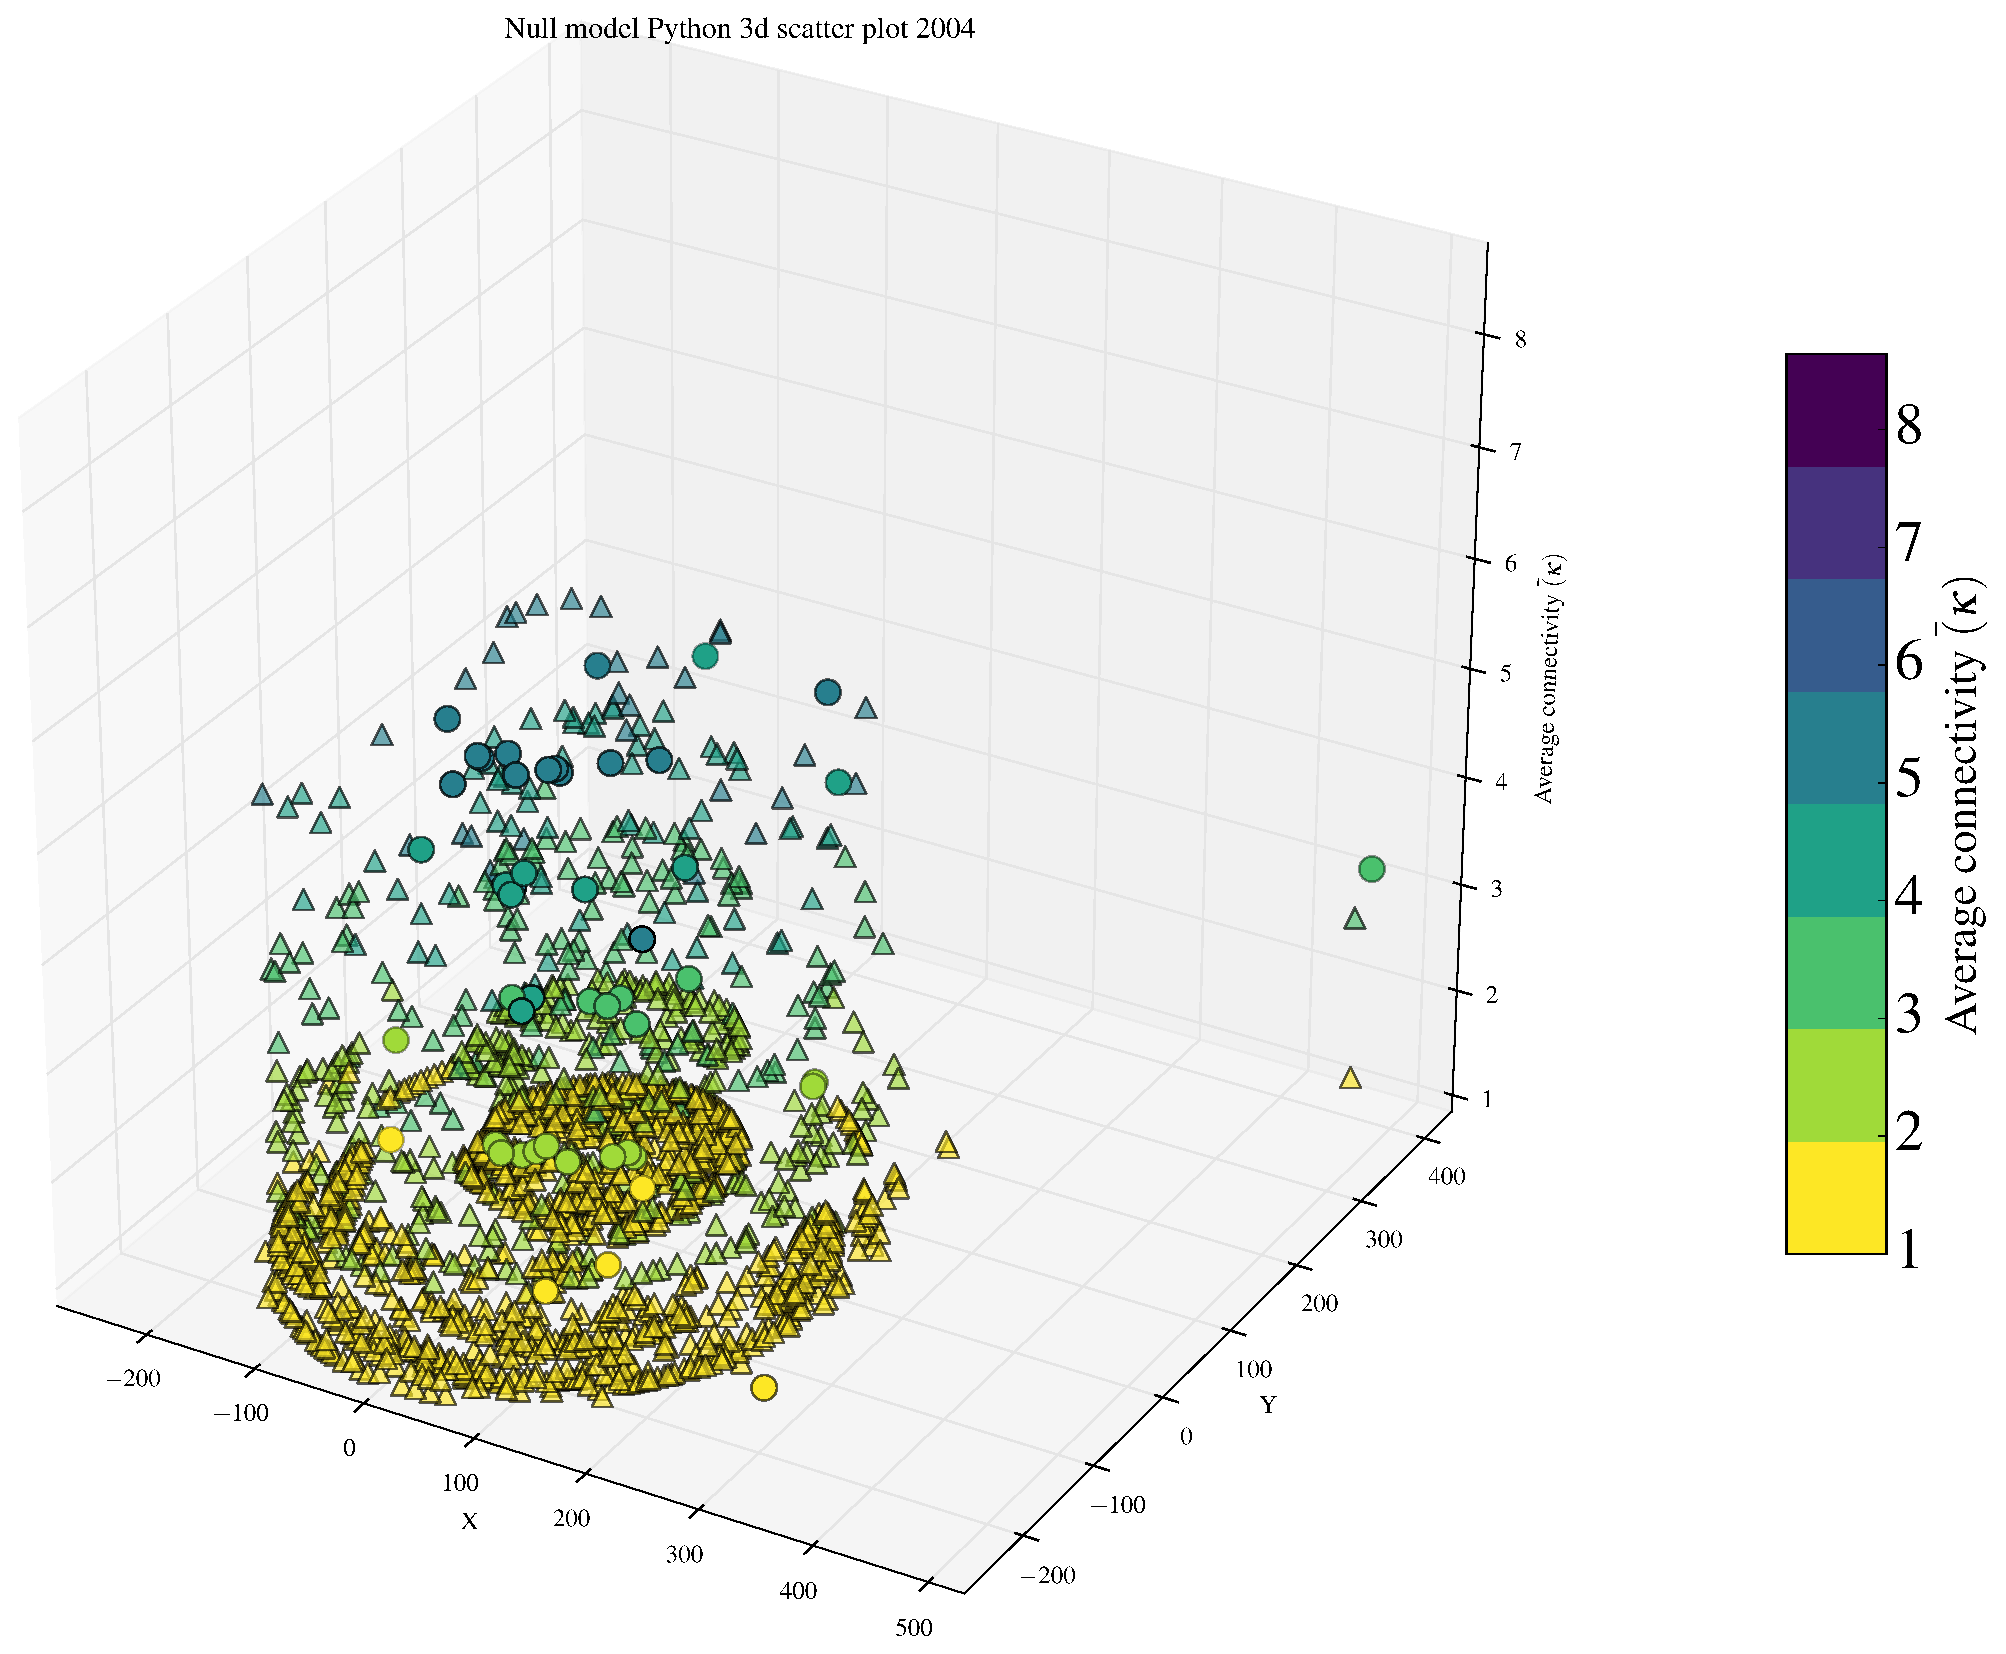
\includegraphics[scale=0.23]{figures/3d_scatter_python_2004_null}
}

\subfloat[Actual Python network 2013]{
\label{fig:s3d_actual_python_2013}
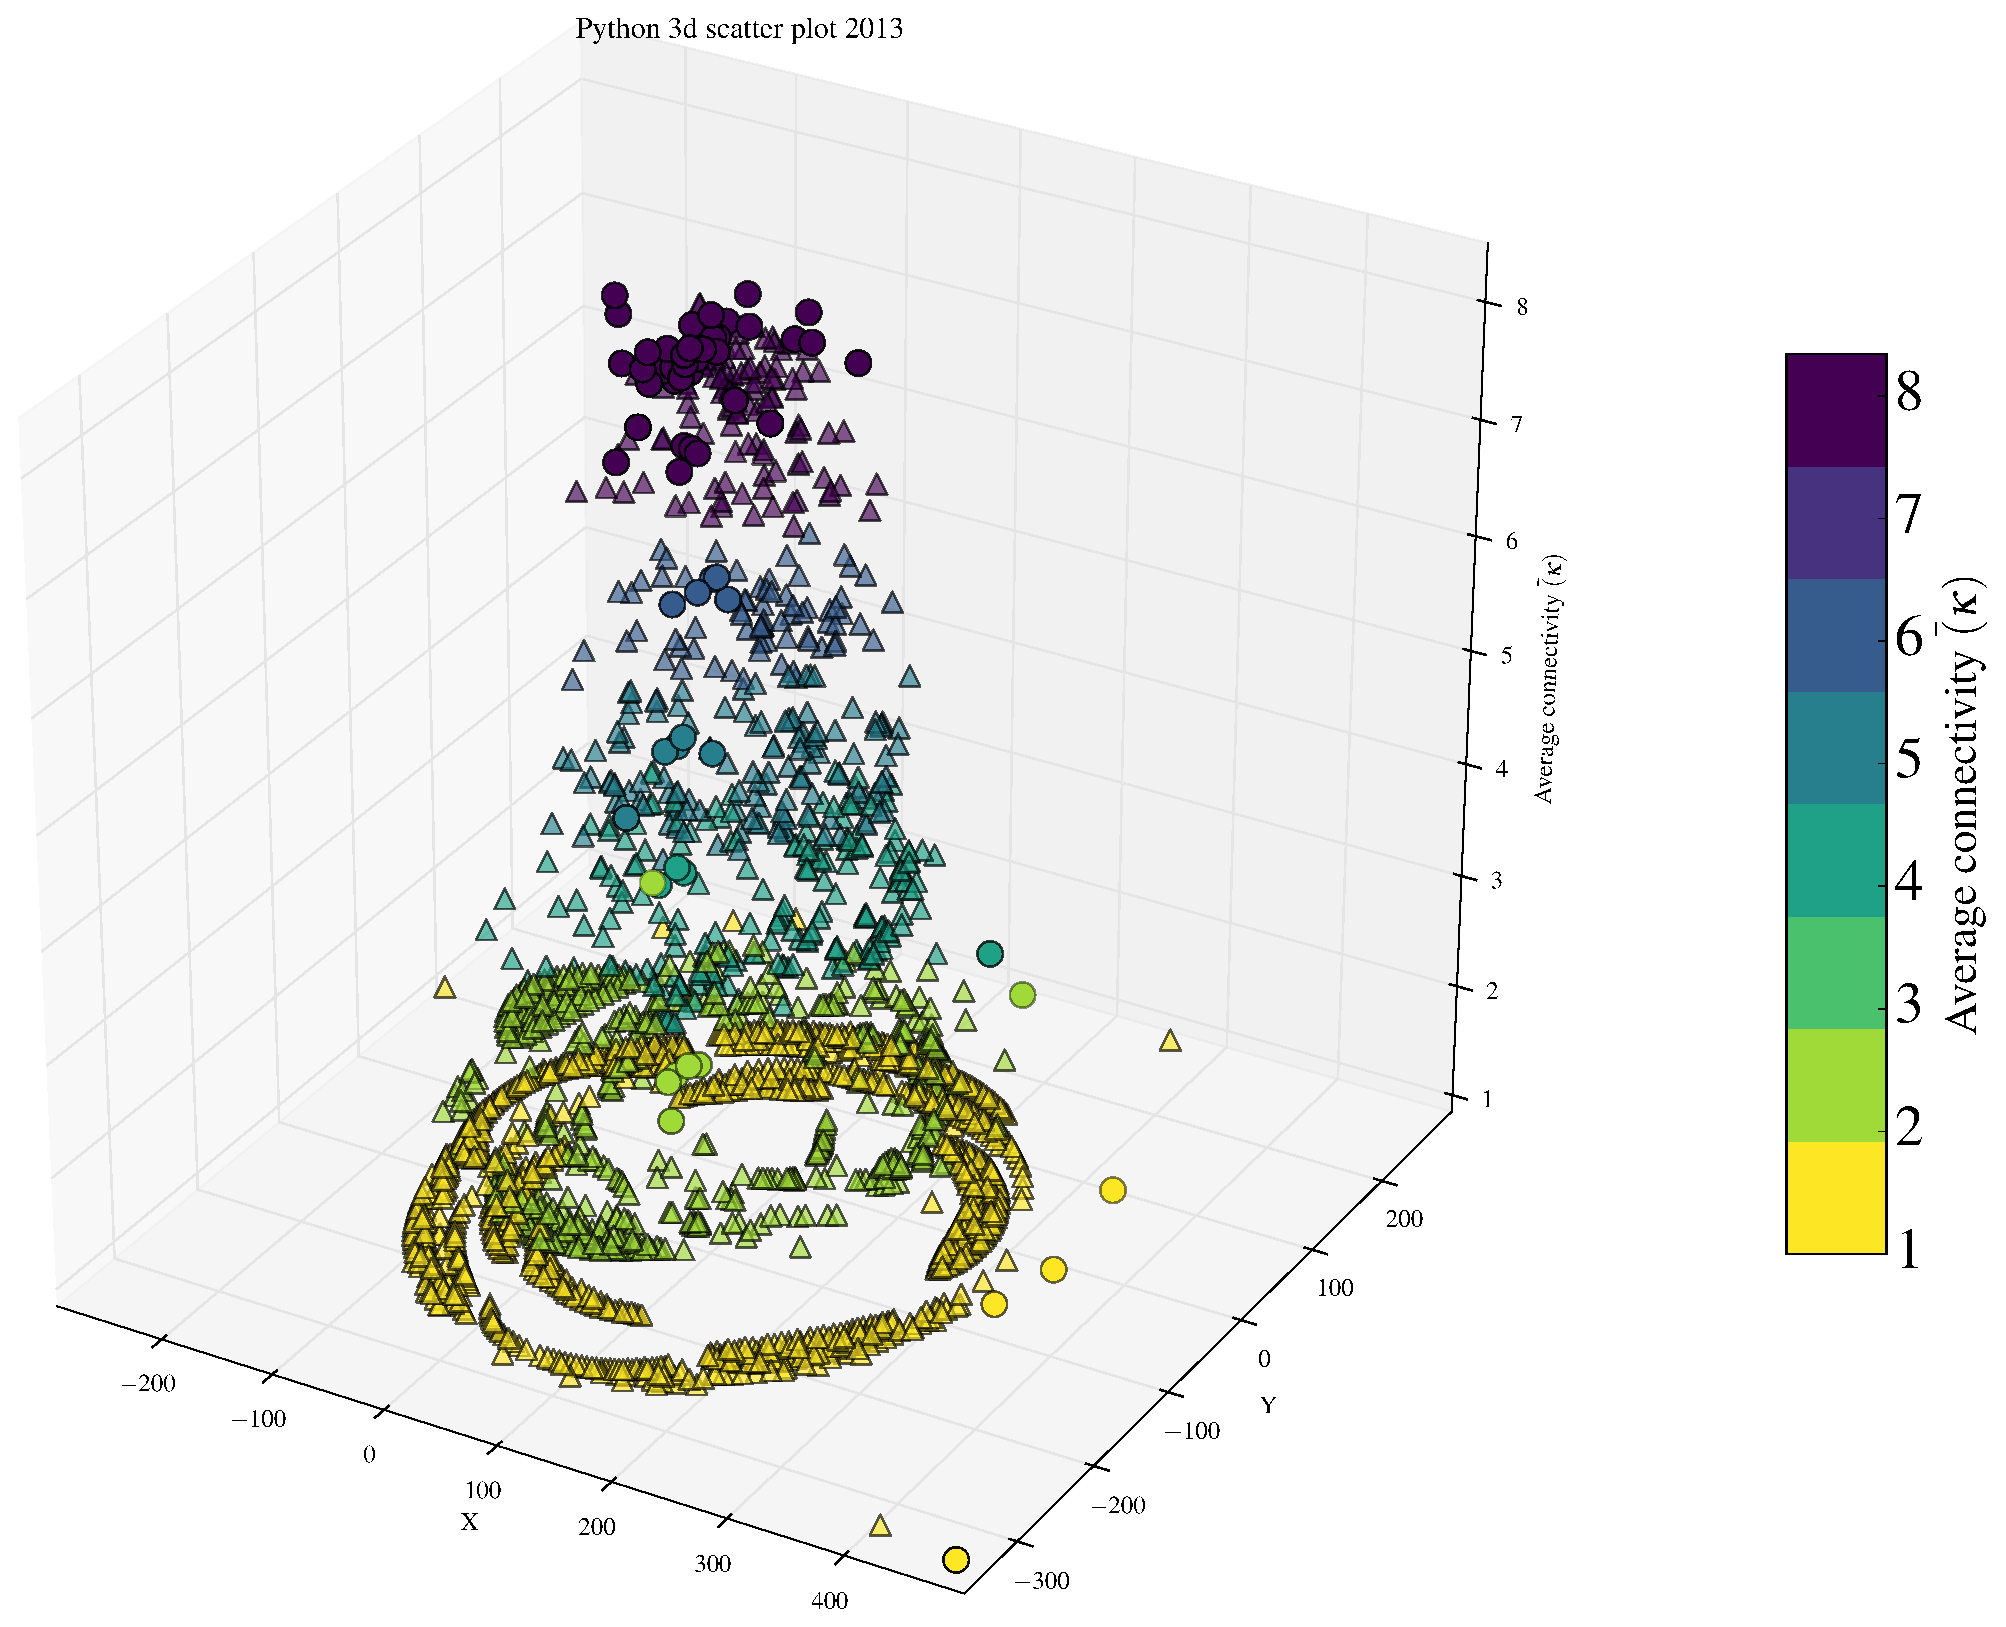
\includegraphics[scale=0.23]{figures/3d_scatter_python_2013}
}
\hspace{.01in}
\subfloat[Null model Python network 2013]{
\label{fig:s3d_null_python_2013}
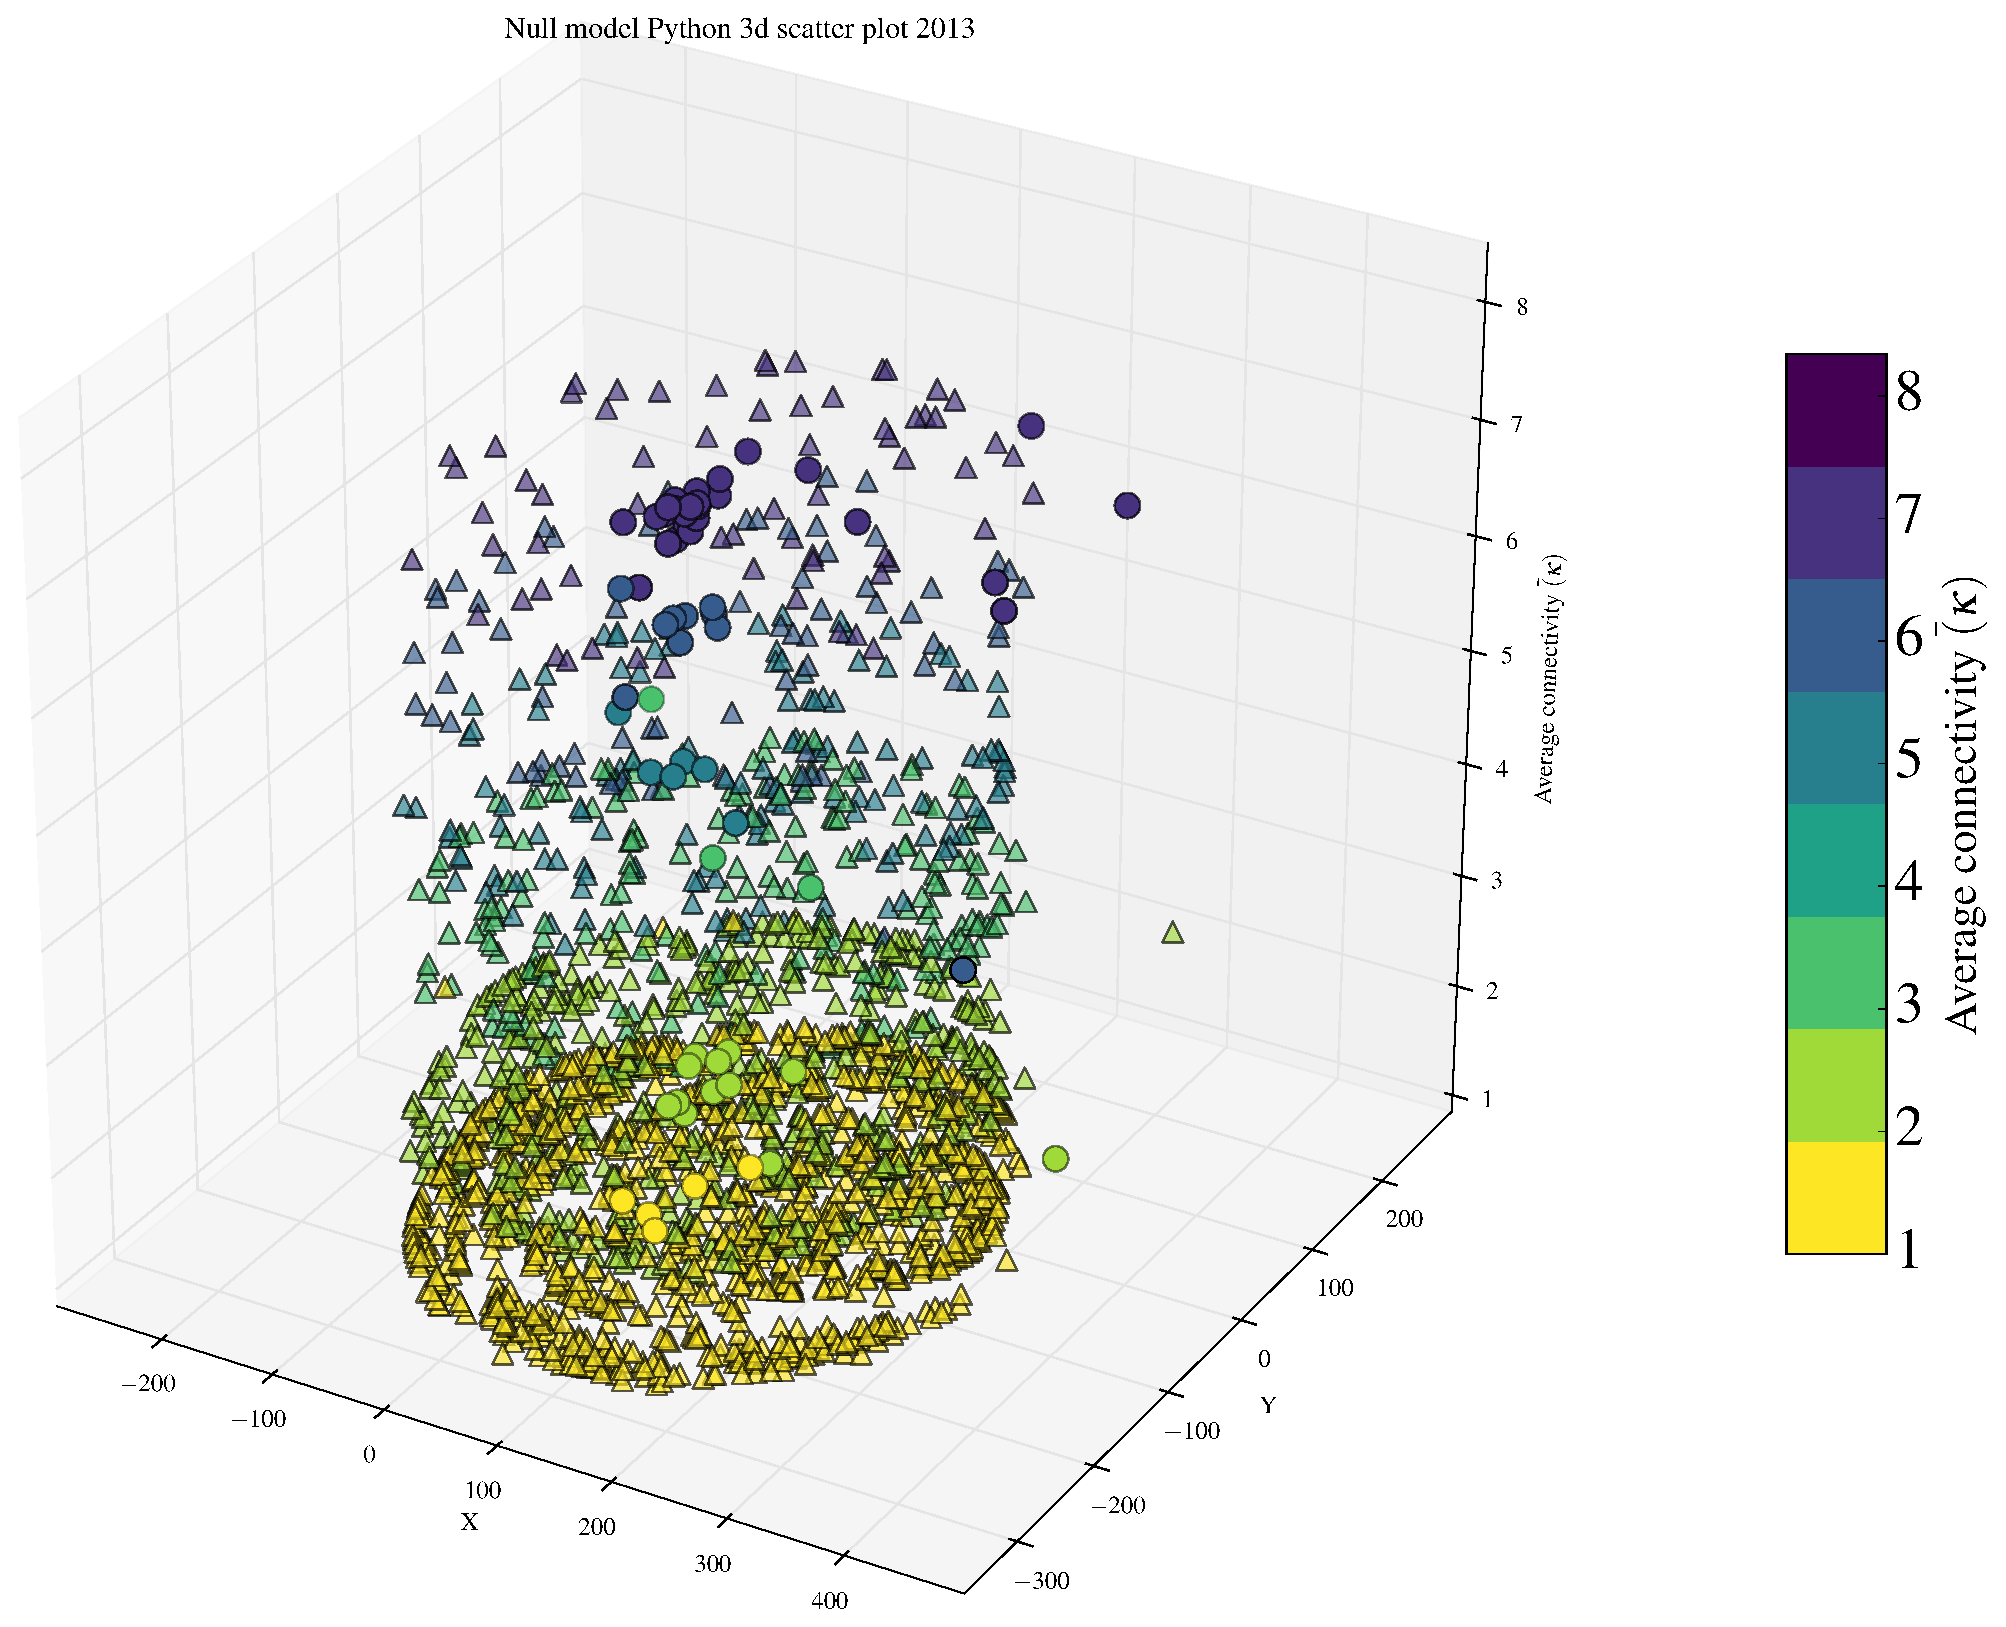
\includegraphics[scale=0.23]{figures/3d_scatter_python_2013_null}
}

\caption[Python average connectivity three-dimensional scatter plots.]{Python average connectivity three-dimensional scatter plots for actual networks and their random null models counterparts. X and Y are the positions determined by the Kamada-Kawai layout algorithm. The vertical dimension is average connectivity. Each mark is a node of the network as two-mode networks they contain both programs (triangles) and developers (circles).}
\label{fig:python-s3d}
\end{figure}


\begin{table}[H]
\begin{center}
\begin{tabular}{|c|c|c|c|c|c|c|c|}
\hline
Years&Nodes&GC&Random GC&GBC&Random GBC&maximum $k$&Random max $k$\\
\hline
1999&3,259&66.6\%&83.4\%&9.4\%&11.4\%&3 (0.2\%)&2 (11.4\%)\\
2000&3,593&52.5\%&77.8\%&7.0\%&10.7\%&3 (0.2\%)&2 (10.7\%)\\
2001&5,943&71.6\%&86.4\%&13.9\%&17.5\%&3 (0.1\%)&2 (17.5\%)\\
2002&6,857&72.4\%&88.1\%&12.7\%&17.0\%&4 (0.2\%)&2 (17.0\%)\\
2003&7,276&75.6\%&89.5\%&14.8\%&20.2\%&5 (0.2\%)&2 (20.2\%)\\
2004&7,984&78.4\%&94.4\%&22.1\%&27.7\%&5 (0.2\%)&2 (27.7\%)\\
2005&8,328&83.8\%&94.4\%&26.1\%&31.3\%&4 (0.5\%)&3 (4.5\%)\\
2006&9,599&84.2\%&96.7\%&33.7\%&39.0\%&4 (0.6\%)&3 (8.4\%)\\
2007&9,471&86.5\%&96.1\%&35.6\%&40.7\%&4 (0.2\%)&3 (8.6\%)\\
2008&10,662&87.2\%&96.4\%&34.3\%&40.3\%&4 (0.6\%)&3 (7.5\%)\\
2009&11,336&89.4\%&96.1\%&35.7\%&42.3\%&5 (0.4\%)&3 (8.2\%)\\
2010&10,515&86.9\%&95.5\%&32.7\%&39.8\%&5 (0.2\%)&3 (5.1\%)\\
2011&12,362&87.7\%&95.0\%&30.6\%&36.0\%&5 (0.3\%)&3 (5.3\%)\\
2012&11,904&87.1\%&95.0\%&31.0\%&36.7\%&4 (0.1\%)&3 (2.3\%)\\
\hline
\end{tabular}
\caption{Structural Cohesion metrics for debian networks.}
\label{str_cohesion_debian}
\end{center}
\end{table}




\begin{figure}[p]
%\centering
\subfloat[Actual Debian network 2000]{
\label{fig:s3d_actual_debian_2000}
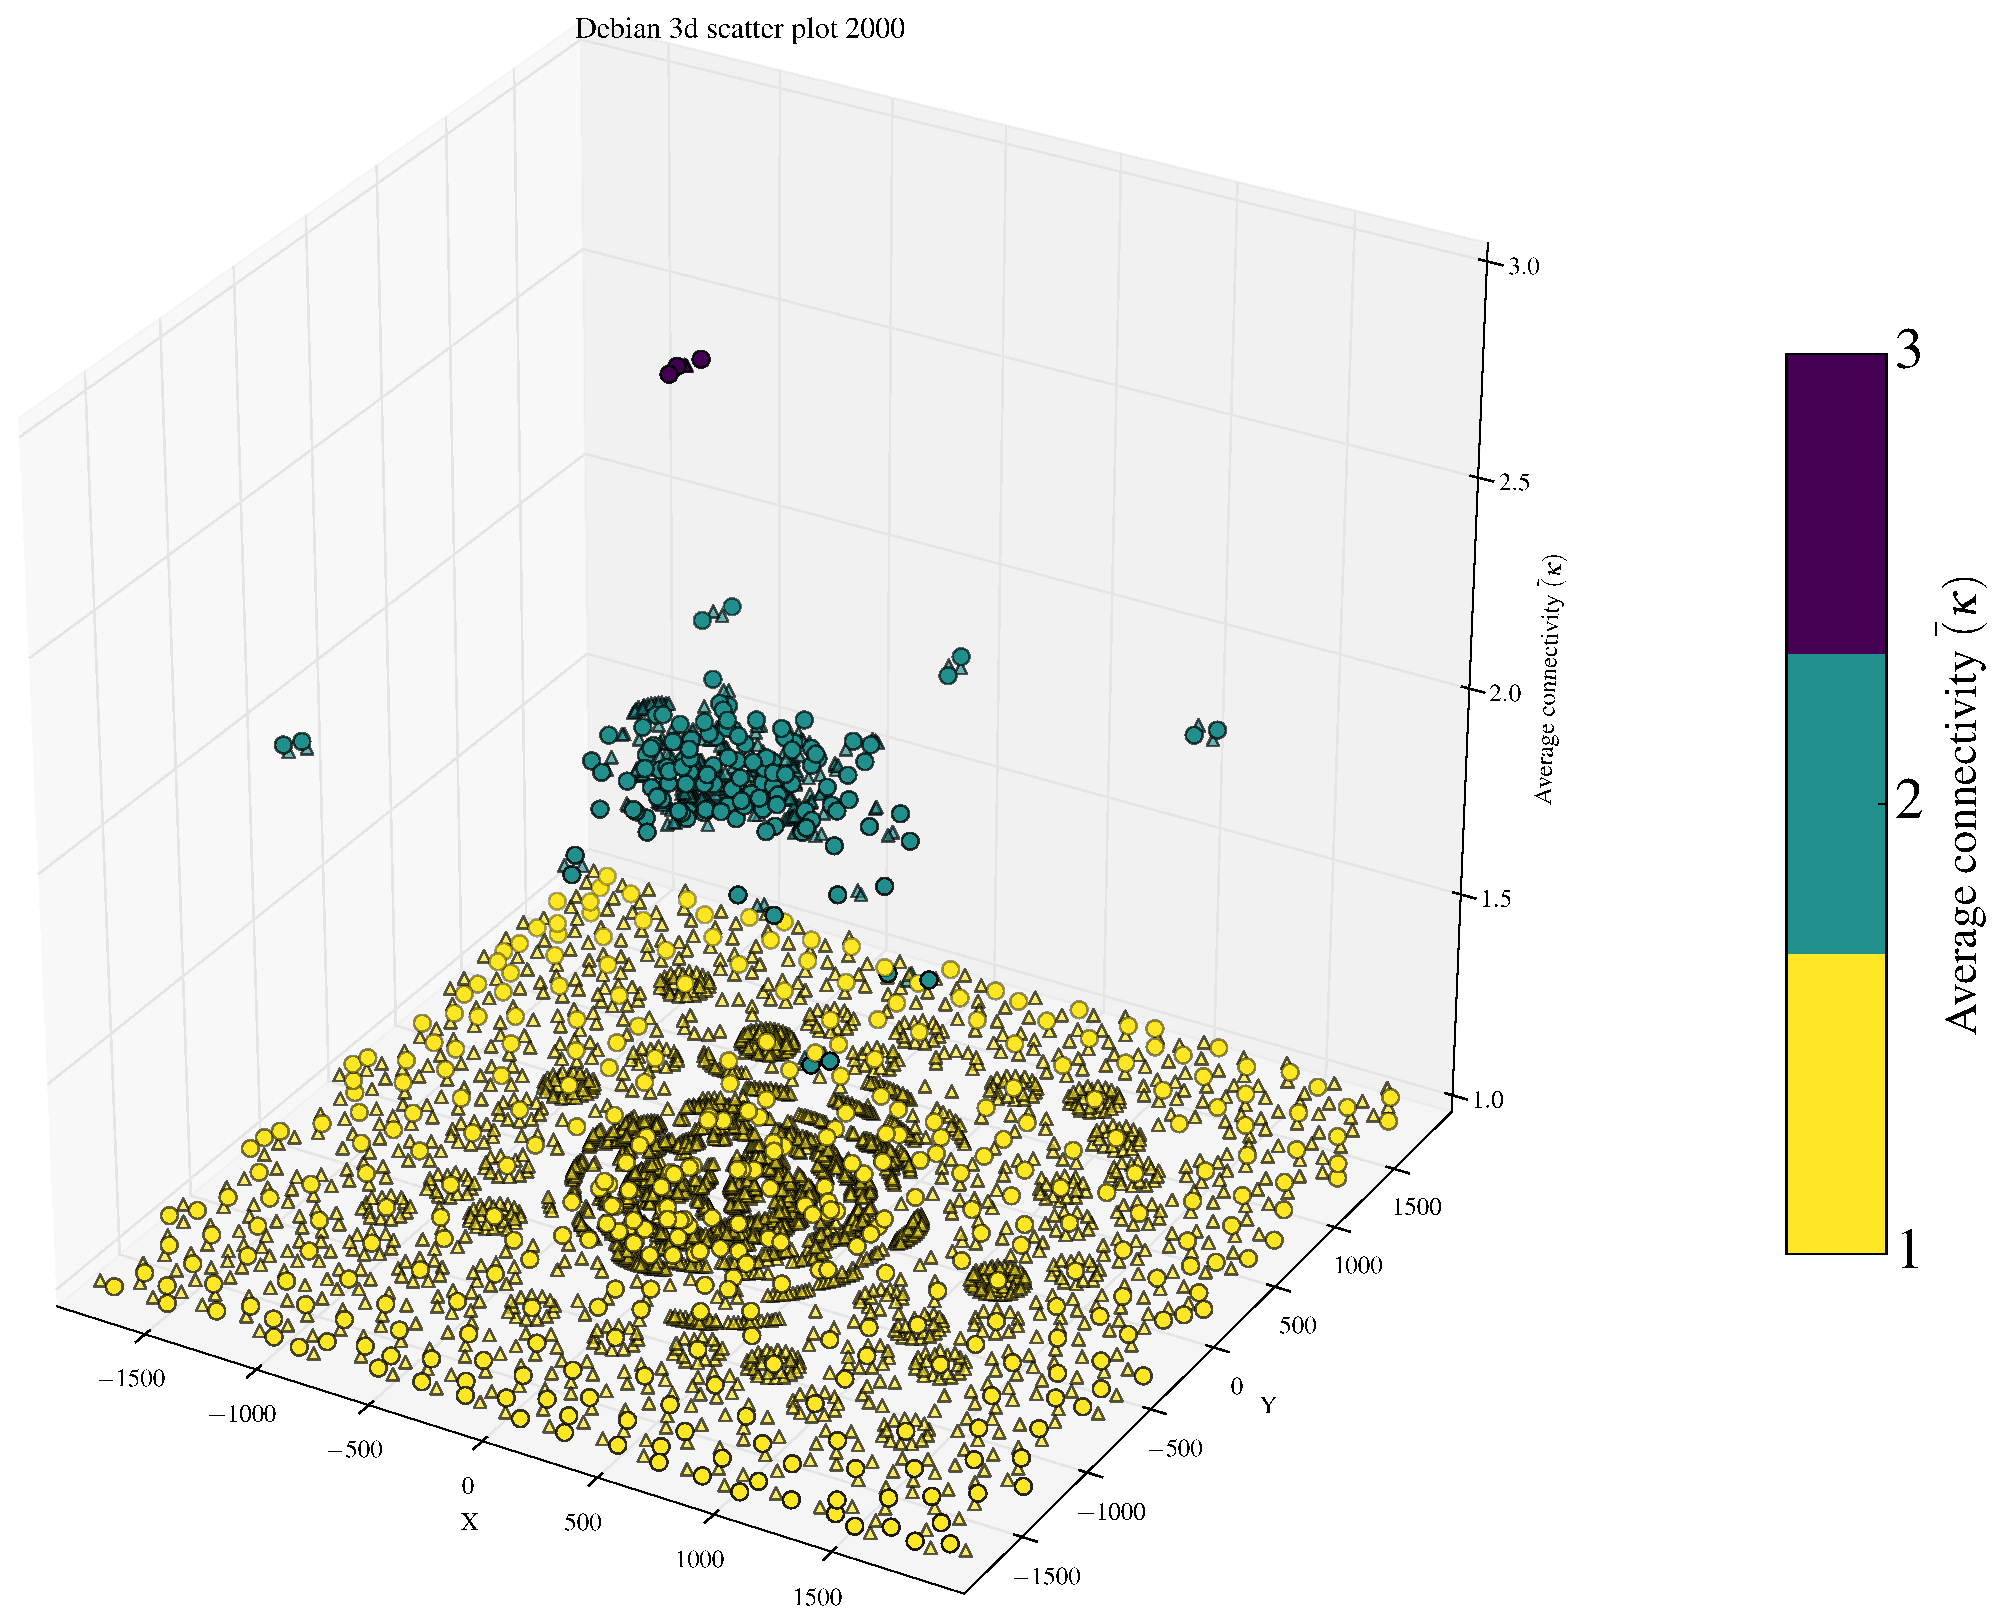
\includegraphics[scale=0.23]{figures/3d_scatter_debian_2000}
}
\hspace{.01in}
\subfloat[Null model Debian network 2000]{
\label{fig:s3d_null_debian_2000}
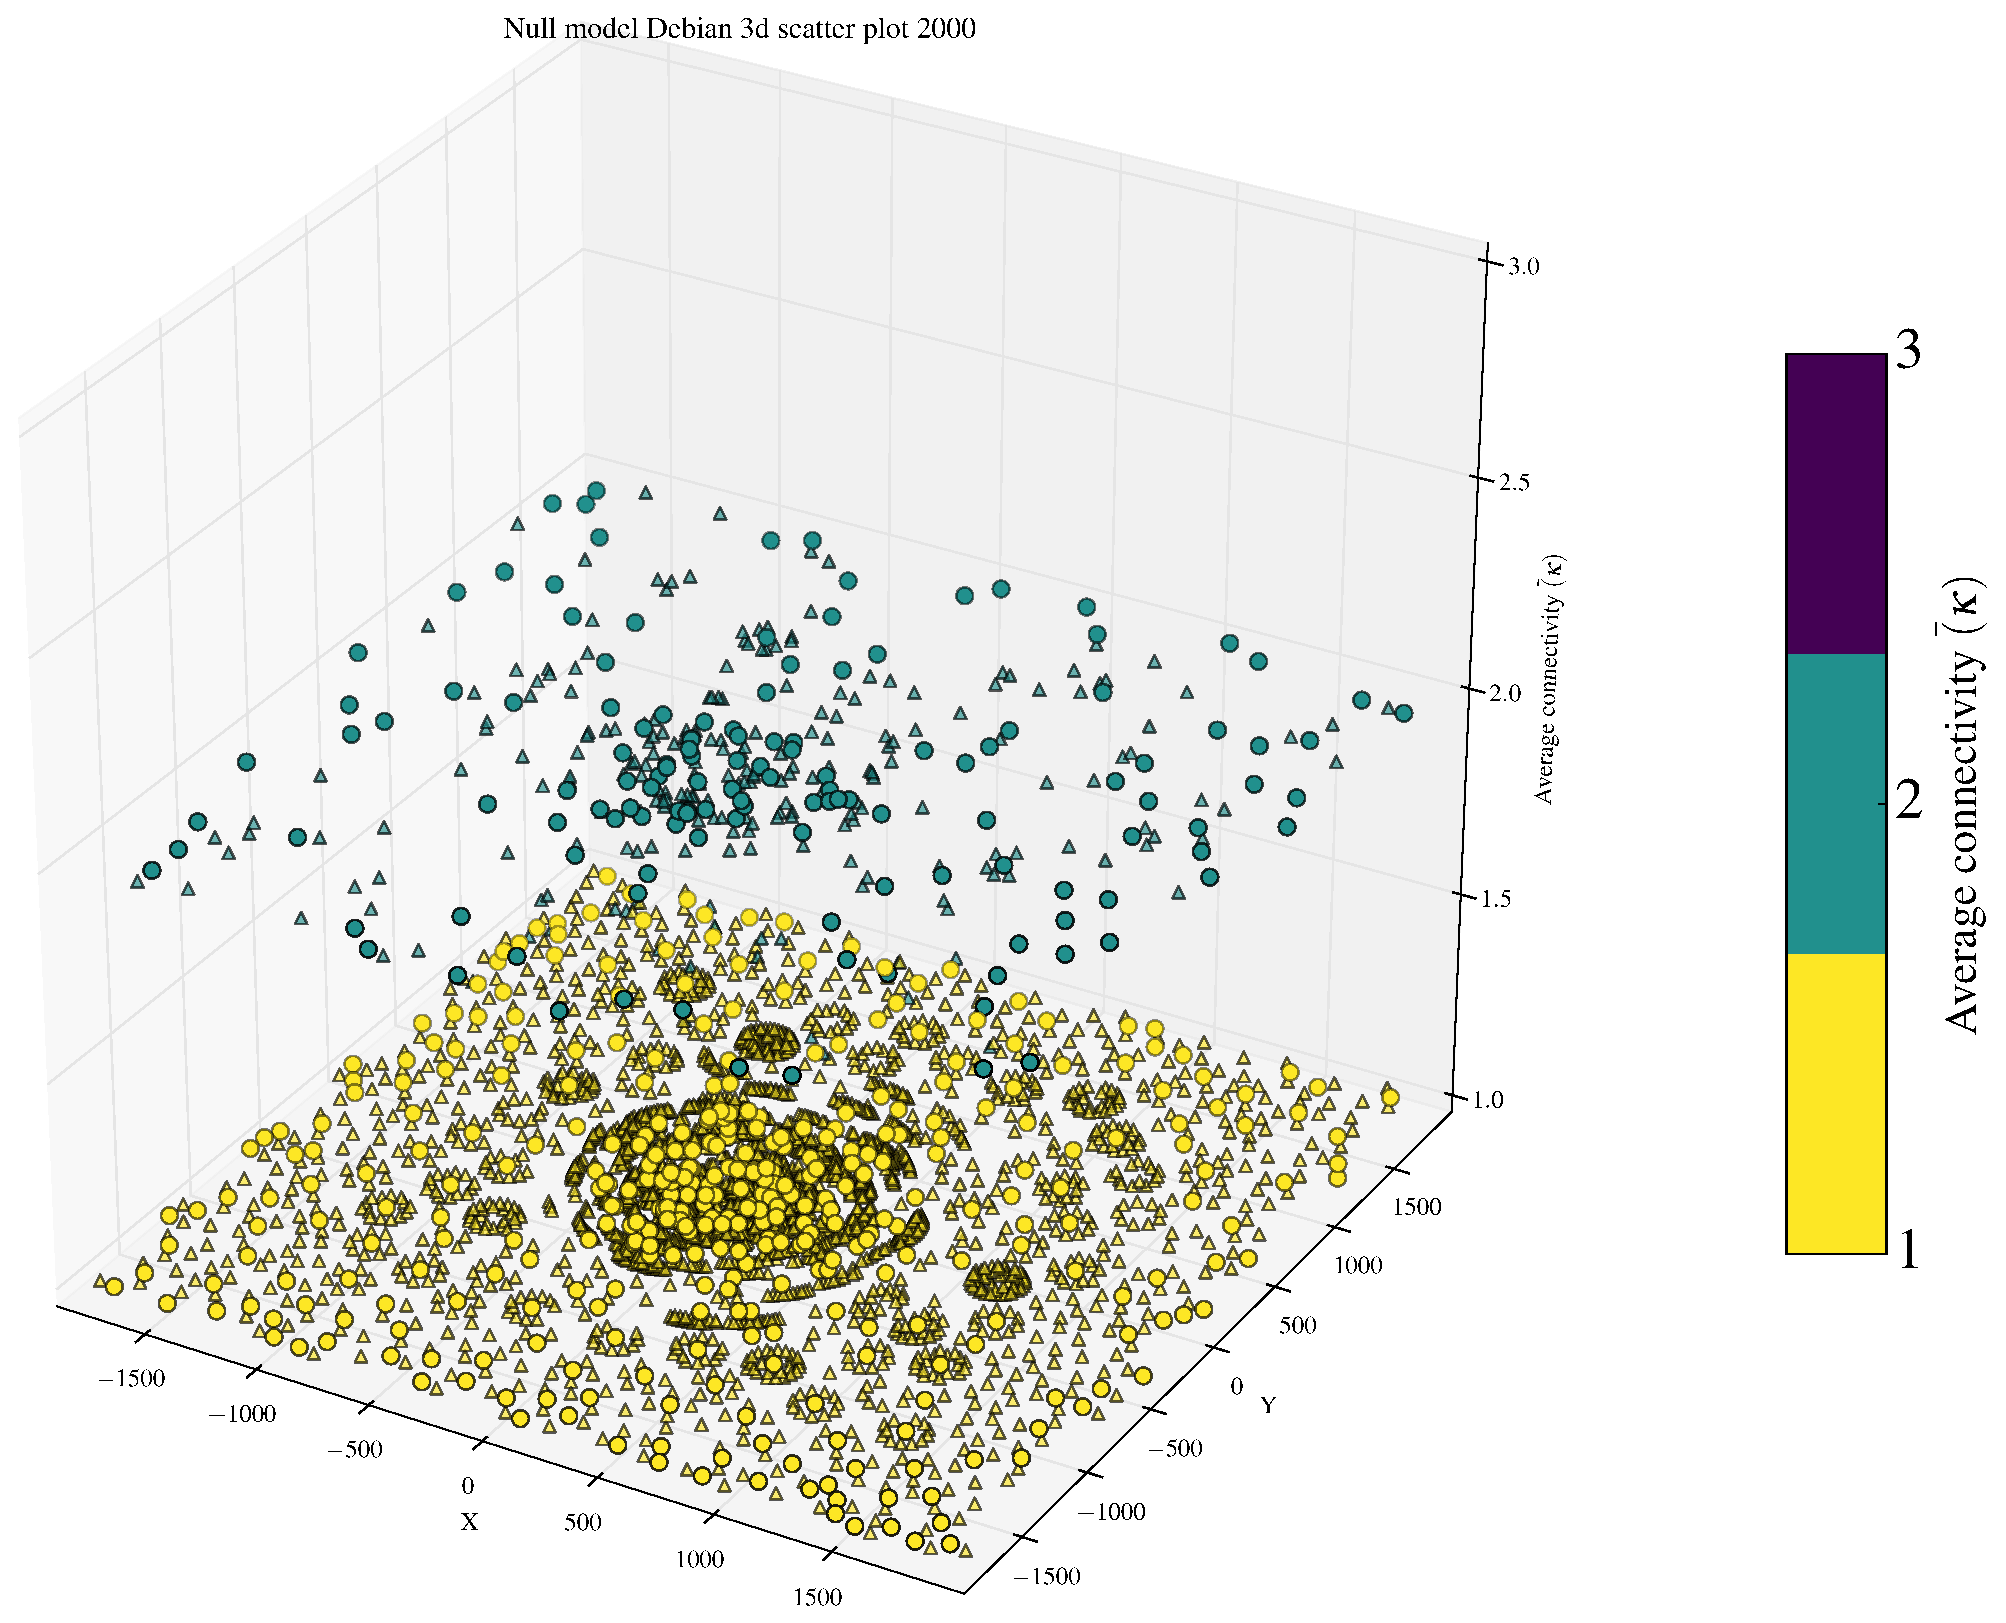
\includegraphics[scale=0.23]{figures/3d_scatter_debian_2000_null}
}

\subfloat[Actual Debian network 2004]{
\label{fig:s3d_actual_debian_2004}
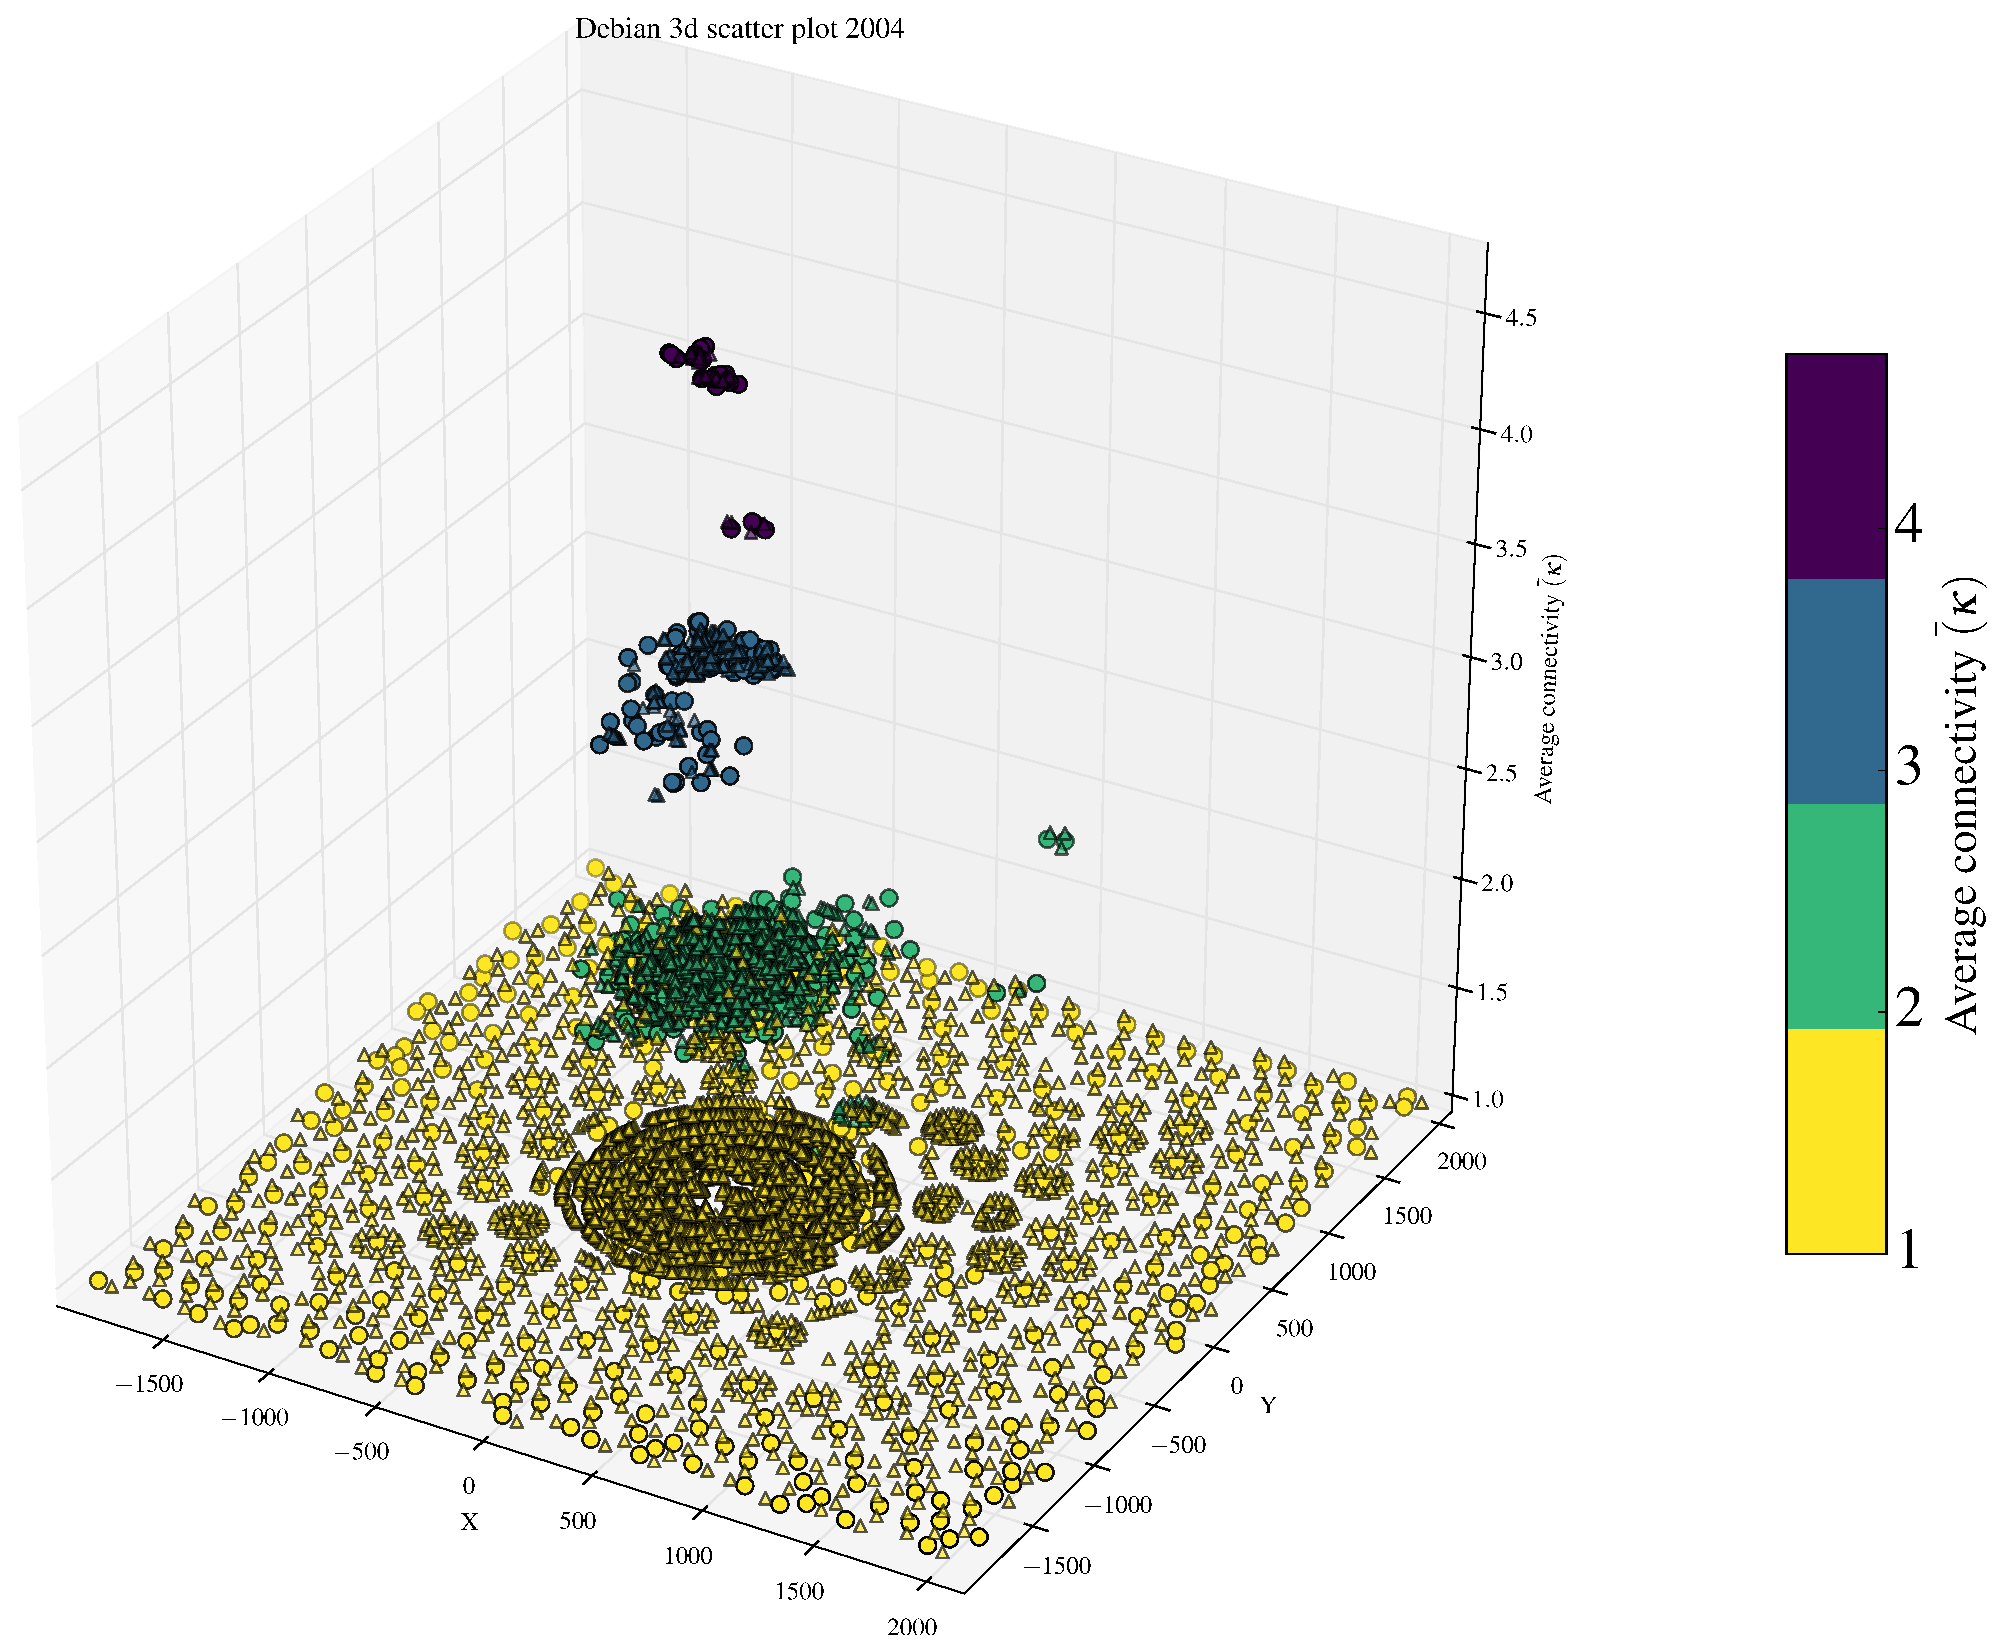
\includegraphics[scale=0.23]{figures/3d_scatter_debian_2004}
}
\hspace{.01in}
\subfloat[Null model Debian network 2004]{
\label{fig:s3d_null_debian_2004}
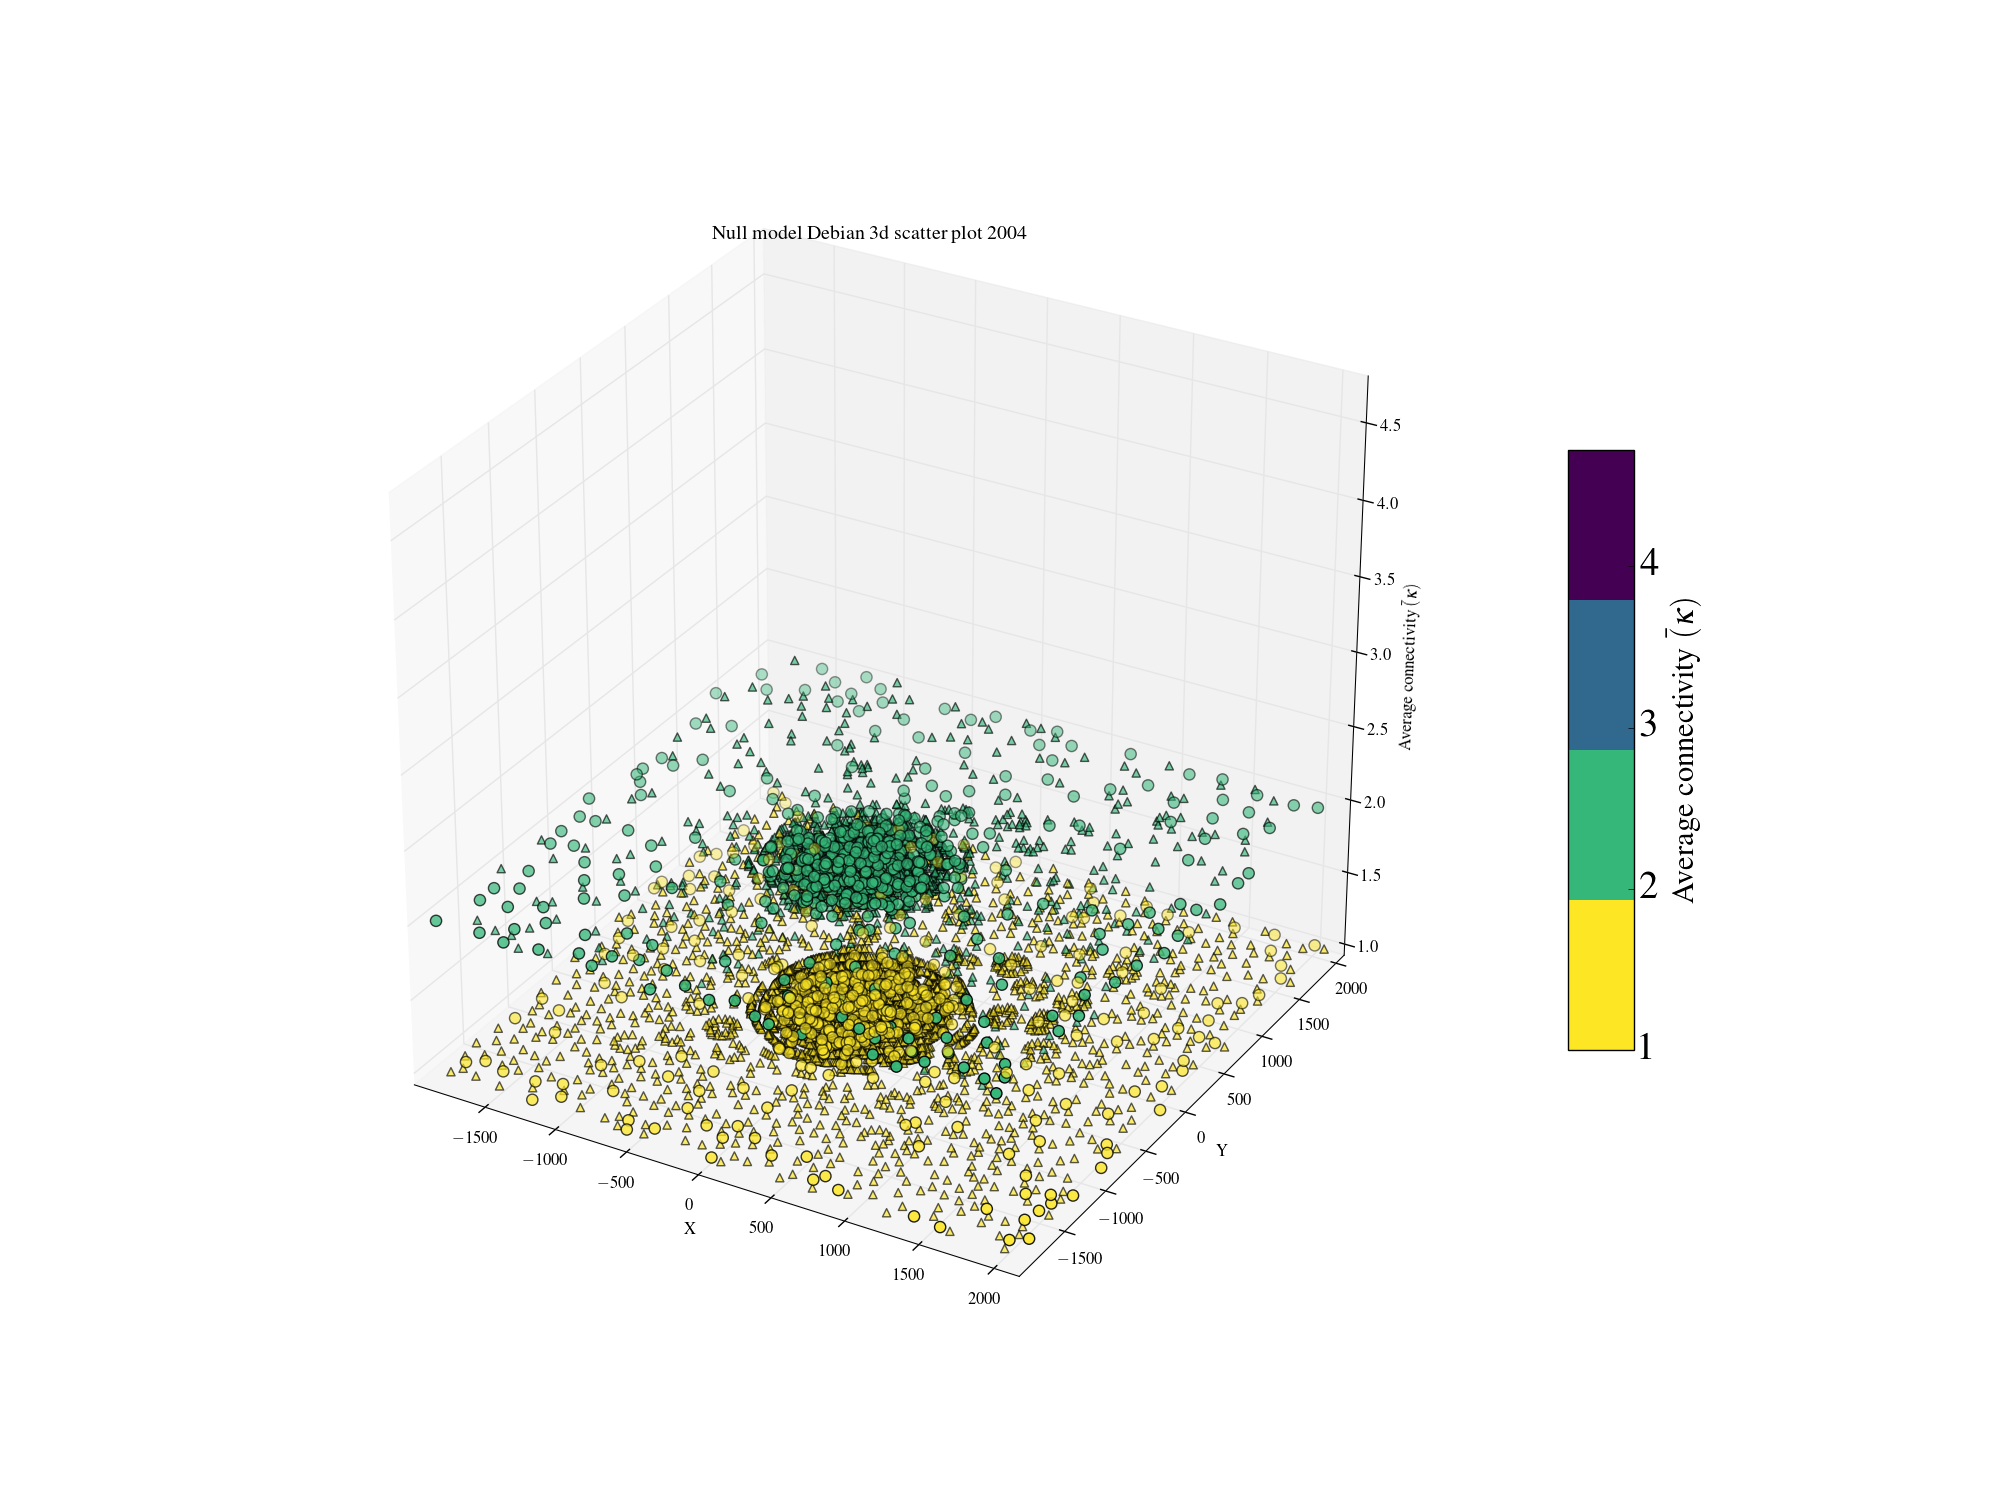
\includegraphics[scale=0.23]{figures/3d_scatter_debian_2004_null}
}

\subfloat[Actual Debian network 2011]{
\label{fig:s3d_actual_debian_2011}
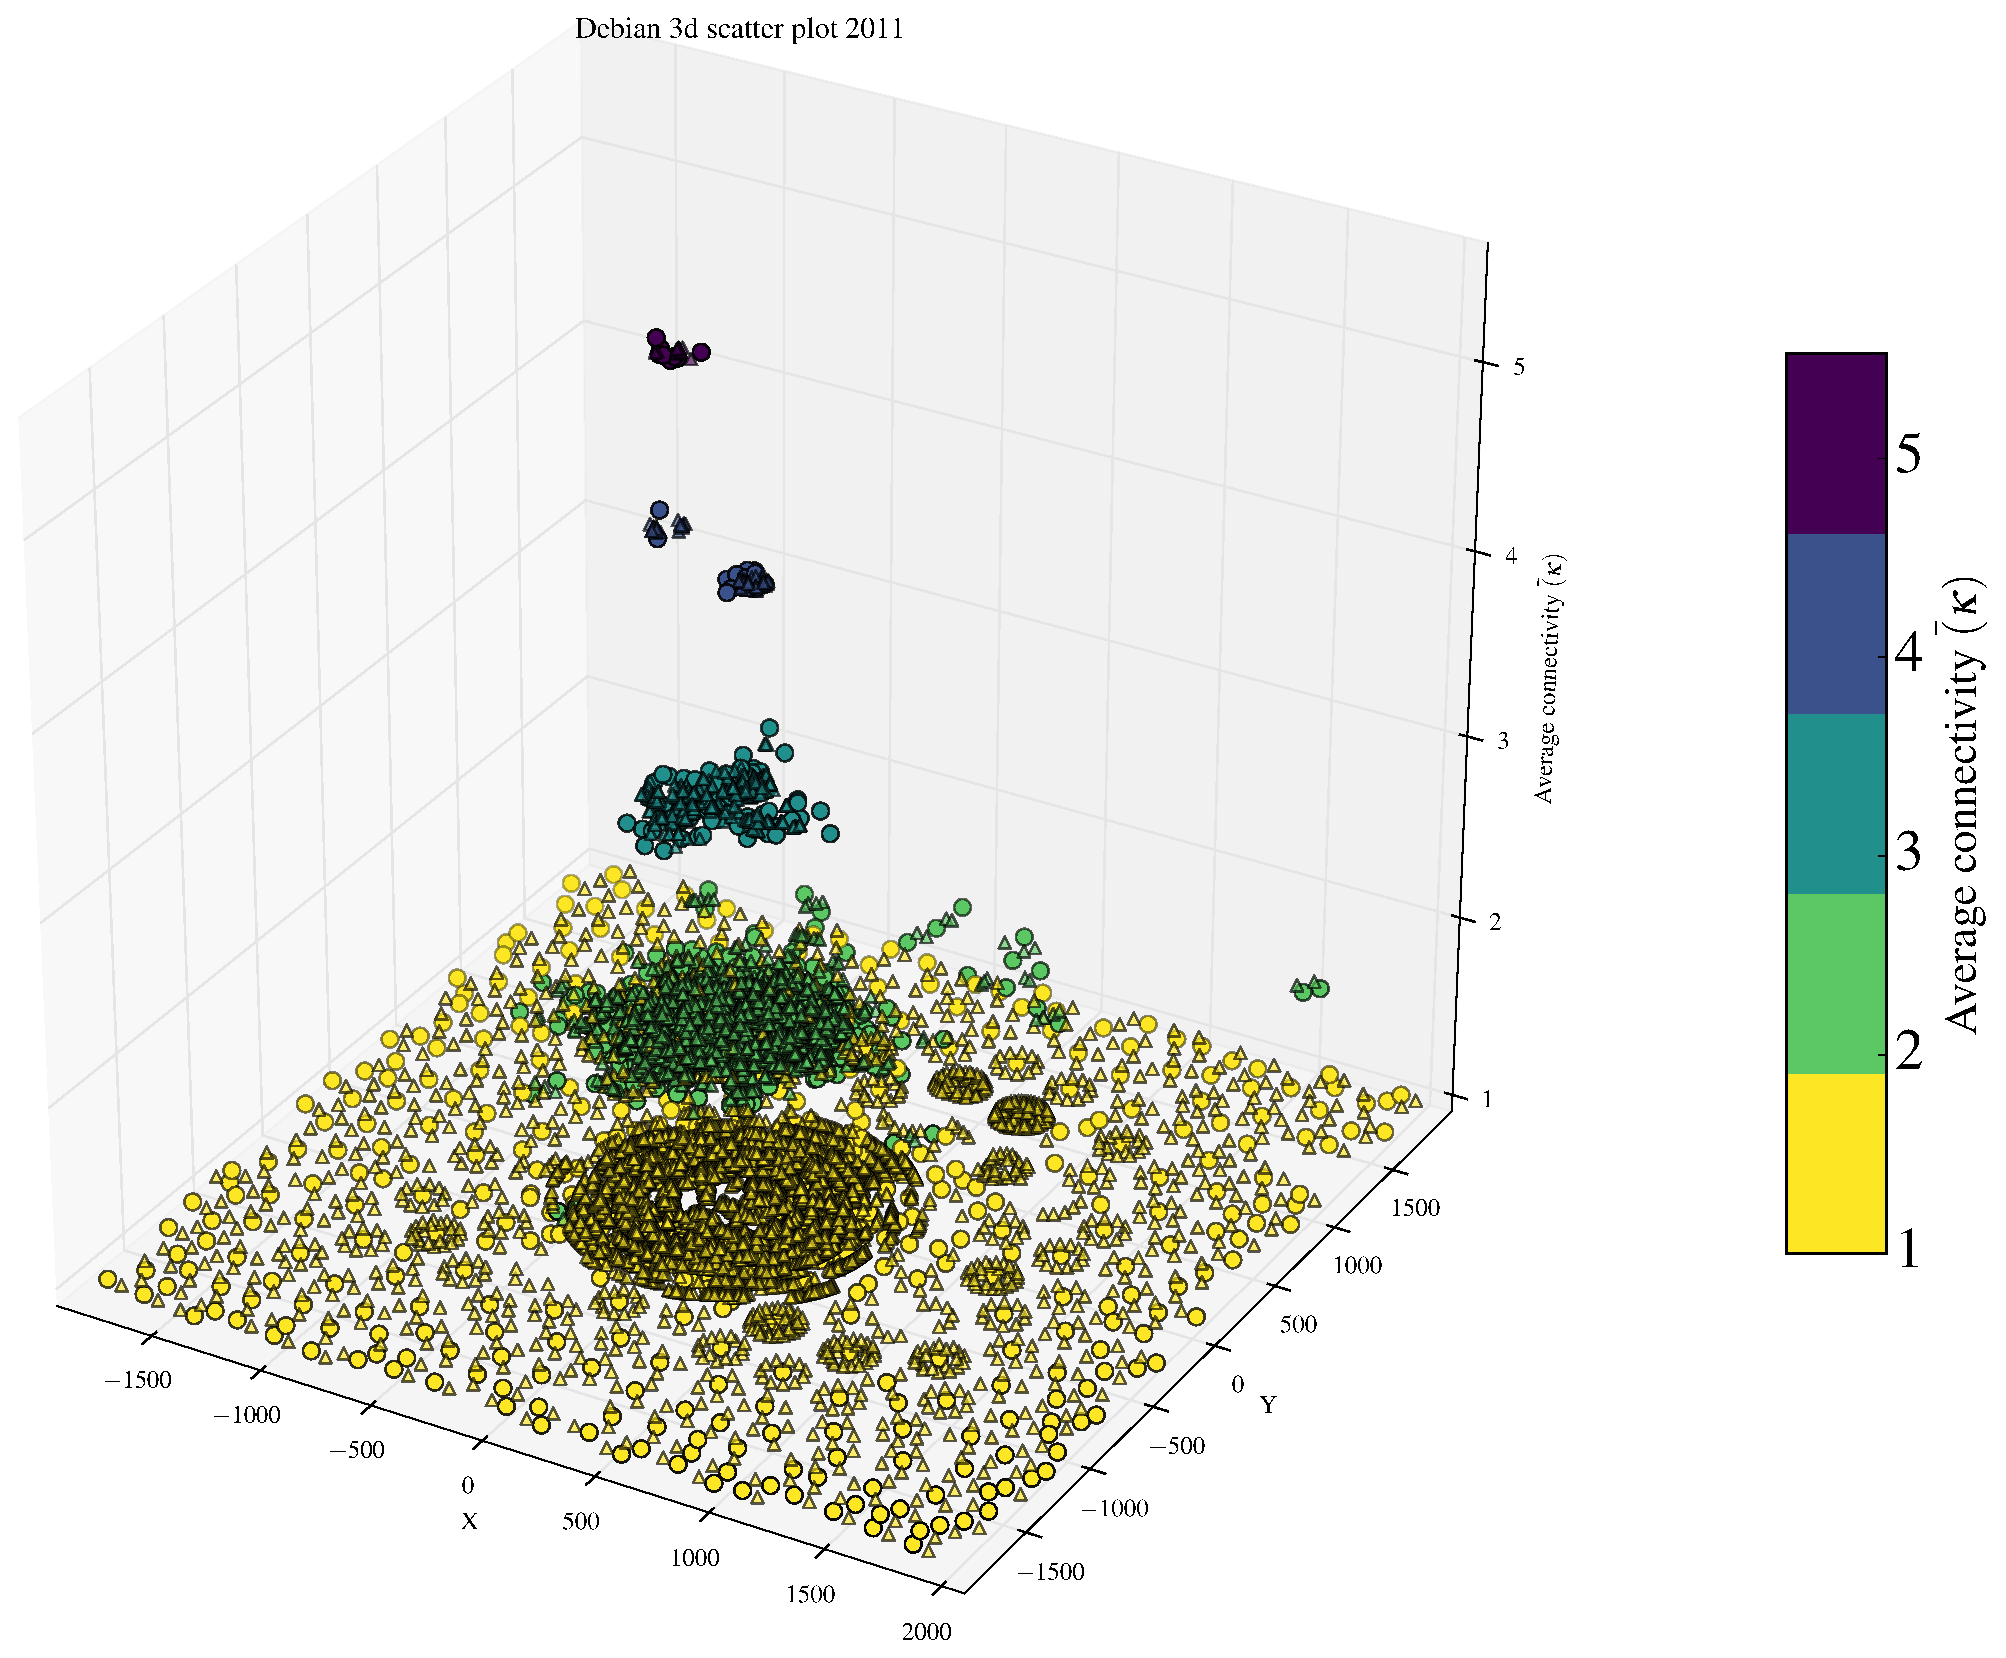
\includegraphics[scale=0.23]{figures/3d_scatter_debian_2011}
}
\hspace{.01in}
\subfloat[Null model Debian network 2011]{
\label{fig:s3d_null_debian_2011}
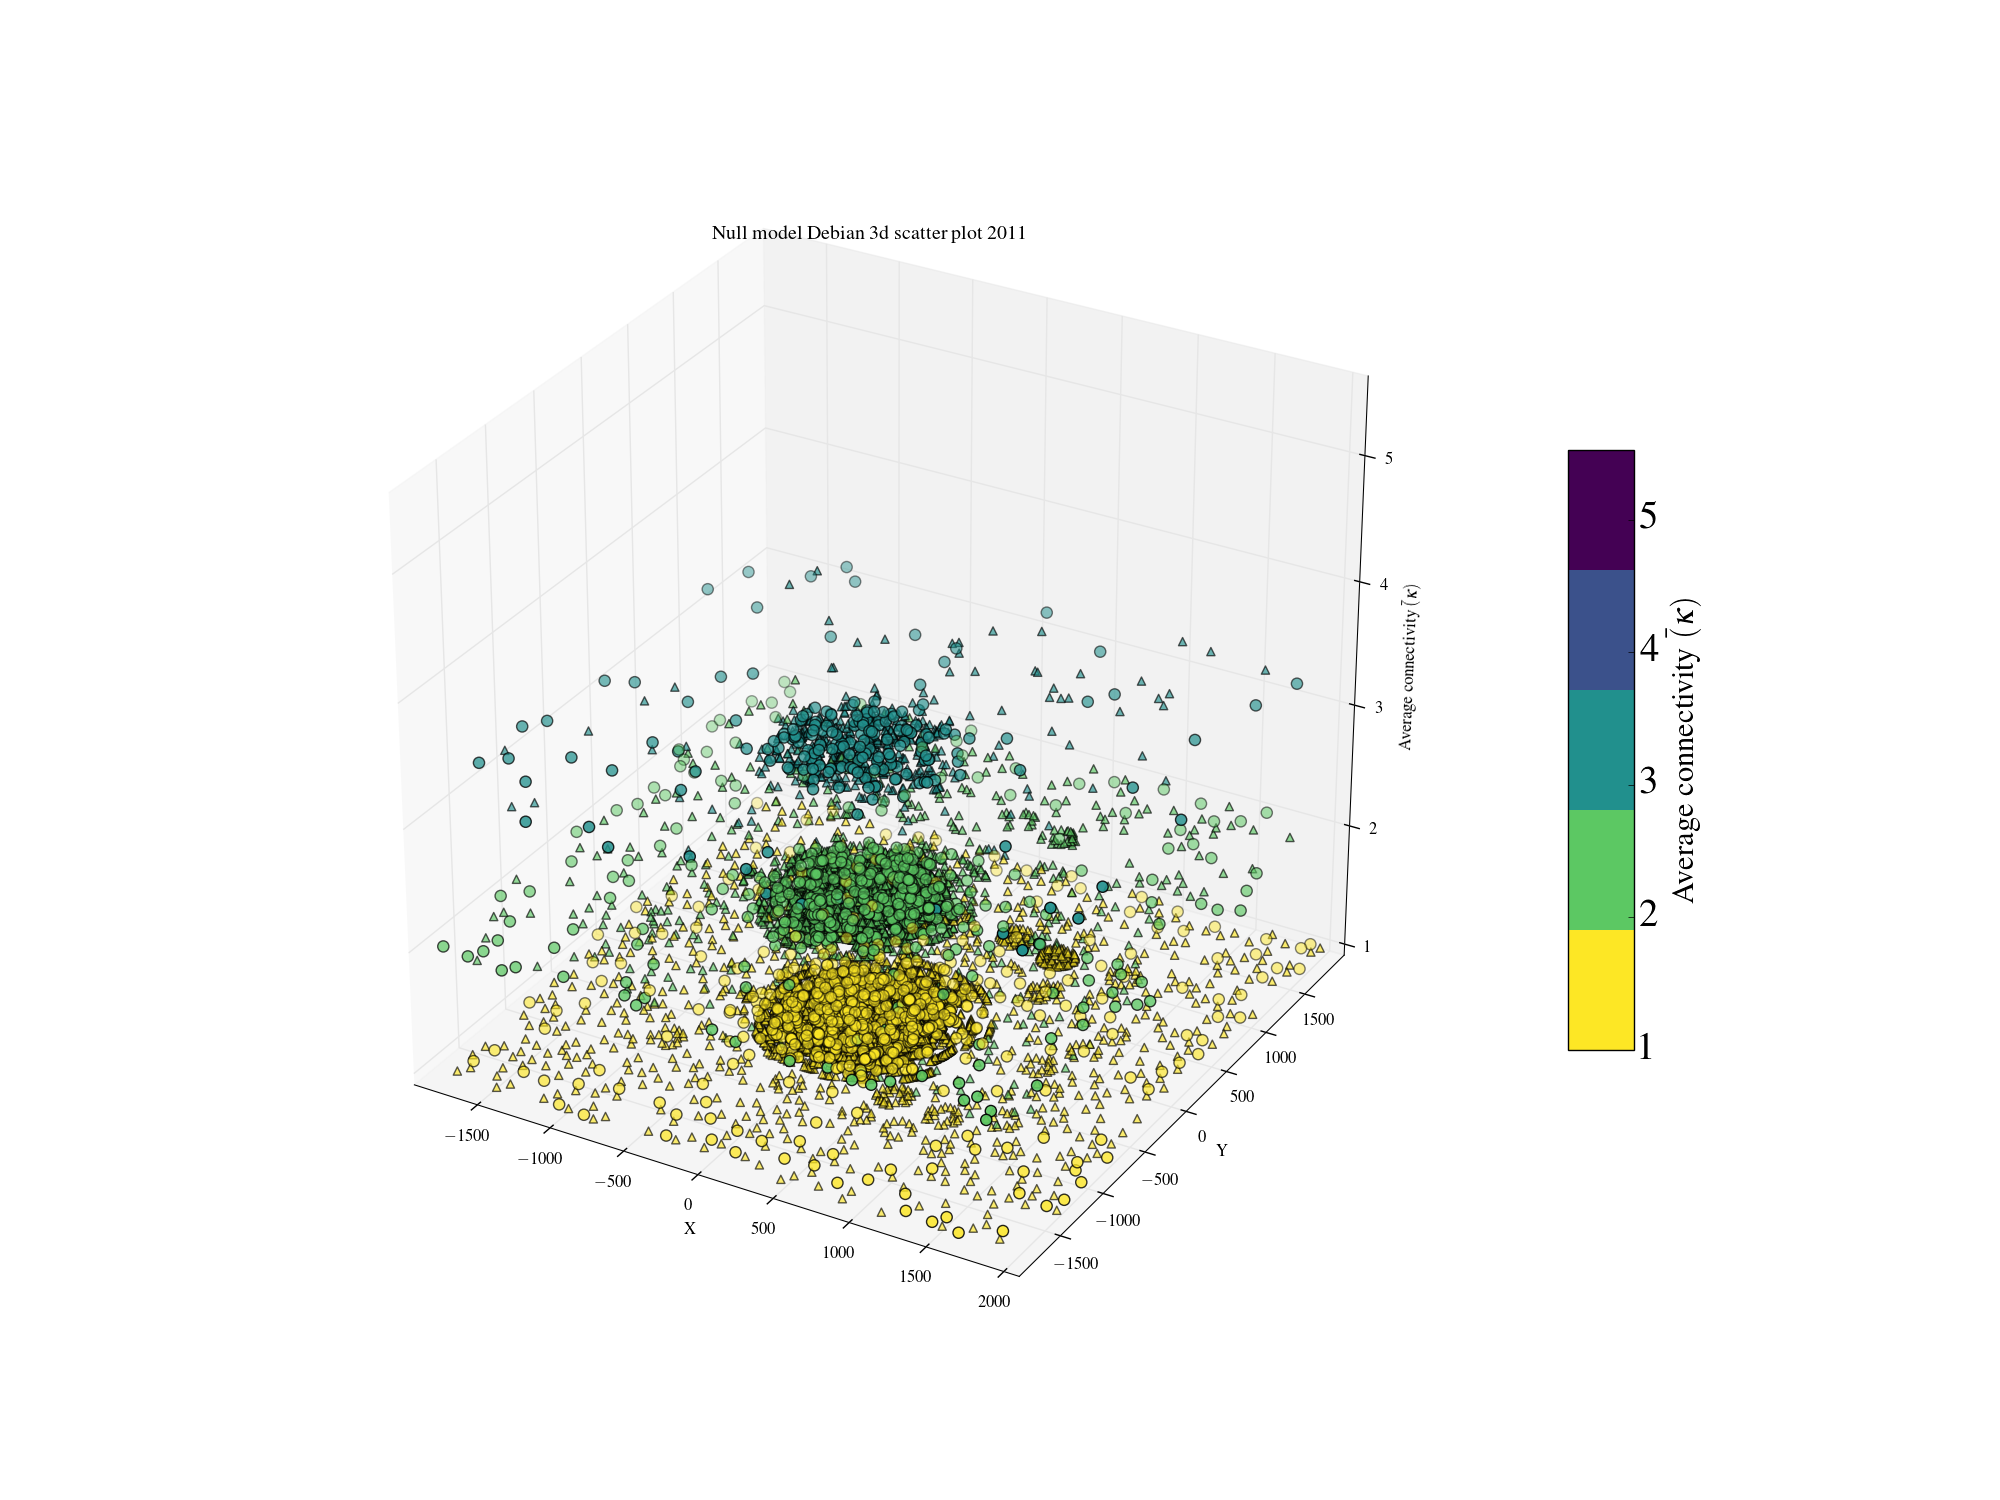
\includegraphics[scale=0.23]{figures/3d_scatter_debian_2011_null}
}

\caption[Debian average connectivity three-dimensional scatter plots.]{Debian average connectivity three-dimensional scatter plots for actual networks and their random null models counterparts. X and Y are the positions determined by the Kamada-Kawai layout algorithm. The vertical dimension is average connectivity. Each mark is a node of the network as two-mode networks they contain both programs (triangles) and developers (circles).}
\label{fig:debian-s3d}
\end{figure}

